In \runone all \veloTracks in \hltone were filtered by the \mvm algorithm. The latter performs a quick check,
given the muon stations hits, on wheather a \veloTrack is comaptible with being identified as a muon by the subsecuent
tracking algorithms, before these algorithms are actualy run. If the \veloTrack passes certain simple requirements it
is accepted, otherwise it is discarded permanently and not processed further by the \hlt muon lines. As a result
valuable computing time is saved, since the \FwD tracking and fiting algorithms are time costly.

\subsection{The MatchVeloMuon algorithm}
\label{sec:muon_matching}

The \mvm alogorithm, as it was implemented for \runone \cite{roelThesis}, takes a VELO track{\color{red} define velo track} as input
and searches for hits inside a search window, also know as {\it Filed of interest} (FoI), in the M3 muon station.
M3 is the first station to search for hits for two reasons. First the occupancy{\color{red} define} in M2 is very high{\color{red}see roel plot}
thus an initial a single VELO track candidate would create
a huge number of seed hits{\color{red} define seeding}. Second the muon reconstruction algorithm (\isMuon) will always fail if
there is no M3 muon hit asigned to a VELO track.

As it can be seen in \figref{}, the \lhcb magnet is between the \velo tracker and the and muon system.
The \lhcb magnetic field deflects tracks based on their momentum. The lower the momentum of a atrack the more
it is deflected by the magnetic field. Since, no momentum or charge information is available for the \veloTrack
before the \FwD algorithm is run, the size of the M3 FoI is defined assuming a minimum track momentum of 6 \gevc.
This particular momentum value corresponds to the lowest momentum tracks that the subsequent \isMuon algorithm accepts.

After considering all the M3 muons hits inside the FoI, additional muon hits are added to
the M3 seed hits by extrapolating from each M3 seed hit further to the rest of the muon stations.
Since there is no magnetic field between the muons stations the above mentione extrapolations are simple straight lines.
The corresponding FoIs for the rest of the muon stations are smaller since there is no deflection involved.
These FoIs account for the fact that the presence of heavy material between the muon stations change the
trajectory of a muon passing thorough, this effect is called multiple scattering, {\color{red} cite panos or other shit.}
and it is more pronounced for low momentum tracks.

At least 3 hits in the muon stations M2-M5 are required by the \mvm algorithm in order to accept the initial VELO track.
At the end of this procedure all {\it muon candidate tracks} that could result from an initial VELO track were considered.
Within the scope of the current chapter a muon candidate track is defined as the track formed by muon hits only.
Note that at this stage of the algorithm an estimate of the momentum of the initial VELO track becomes available
for each candidate muon track using the kick method \cite{roelThesis}, {\color{red} there is a better citation for that.}.
The kick method provides an estimate of the track momentum given the change in its slope when passing through a magnetic
field of a given streagth. The relation between the change in slope and the track momentum is empiracally estimated
in \cite{roelThesis}.

As a last step the candidate muon tracks originating from the above procedure are filtered by a $\chisq/\nDoF$
requirement. The \chisq is simple to compute since there is no magnetic field in the region of the muon stations
and all tracks are in principle almost straight lines, taking into account the presence of multiple scattering, mentioned above.
The \chisq requirement reduces the chances that random combinations of muon hits can fake a real muon track.
The requirement is particularly usefull for low momentum tracks for which the number of M3 seed hits is larger,
due to larger corresponding M3 FoI, and thus the number of posible random combinations of muon tracks incereases.

An important detail that increases the discriminating power of the above mentioned \chisq requirement is the
so called {\it magnet hit}. The last is not a hit comming from a tracking station but rather the $(x,y)$ coorodinates
of the $z$ focal plane of the \lhcb magnet. The focal plane is essentially the plane defiend by the $z$ coordinate
where the change in the slope of a track, due to the magnetic field,  "instantaneously" takes place. Note that this
instantaneous change in slope is an approximation. In reality the track follows a smooth trajectory inside the whole
area of the amgnetc field, see {\color{red} ecent dispalay}. However estimating this trajectory uses valuable computation time during \hltone, while
\mvm can perform efficiently enough without a smooth track trajectory using the focal pane approximation.
The position of the $z$ focal plane has been studied \cite{} and used in the \mvm algorithm.
As mentioned in the begining of the paragraph including the magnet hit helps rejecting fake muon tracks.
Including the magnet hit in the \chisq essentialy requires that the muon hits are aligned in a straight line that
also passes from the magnet hit, which is true for real muon tracks only.

% The distance between the magnet hit and
% the muon system also plays a role, since the pointing of a fake muon track within a given hit resolution
% , $\sim 10 \m$, compared to the one
% between the muon hits, $\sim 1 \m$.

\subsection{Upgrade to MatchVeloTTMuon}
\label{sec:matchvelottmuon}
As mentioned in \secref{muid_hlt1}, due to the inceased \hltone rate in \runtwo it becomes possible to
remove the \mvm algorithm form the sequence of the \hltone muon lines and upgrade all \veloTracks with $\pt>500 \mevc$ to long tracks and fit them.
Furthermore, another improvement is the use of information from the \ttracker tracker when reconstructing \veloTracks \cite{LHCb-PUB-2015-005}.
Note that, the \ttracker is posistioned close enough to the \lhcb magnet to allow for a first track momentum estimate.
The \ttracker momentum resolution is inferior, $\sim 15\%$, compared to the one of long tracks. However filtering
\veloTracks with \ttracker information increases the purity\footnote{by reducing the number of a type of fake tracks called {\it ghost tracks}, see {\color{red} cite ghost}}.
The above mentioned improvements offer oportunities for reconstructing muons with $\pt<500 \mevc$, hearafter low momenta muons,
by upgrading the old \mvm algorithm. The upgraded alrorithm is used by newlly introdced \hltone muon lines which aim
at reconstructing low \pt muons.

The upgraded \mvTTm algorithm improves in three points with respect to the old \mvm algorithm.
First the newly available momentum, and hence charge, information from the \ttracker is used to open smaller M3 FoIs.
This reduces the number of M3 seed hits and hence increases the purity of the \mvTTm algorithm, since the number of
random combinations that coould fake a muon reduces with the number of M3 seed hits.
Second, the parametrization of the magnet $z$ focal plane as well as the errors on the magnet hit $(x,y)$ coordinates
are tuned using simulated data. Lastly the vertical, non-bending, $y$ plane is included in the \chisq
computation\footnote{Note that the $y$ projection of a track is almost a straight line, since the magnetic field is parallel to the $y$ axis
and thus exherting no force along this direction.}, which was not the case in the old \mvm algoritm.
The last two impovements both incerease the discriminating power of the \chisq.
Lastly, an important caveat arises from the fact that there can be \veloTTracks that they do not have any information from
the \ttracker. These tracks are normal high momentum tracks that pass through the \ttracker station's inner hole
where there is no active detector material. Since there is no reason to discard these tracks the upgraded \mvTTm treats
those tracks as the old \mvm algorithm did\footnote{Meaning that the M3 FoI are big enough to include the posibility for
both positively and negatively charged tracks, see \cite{roelThesis}}.

\begin{figure}[t]
  \centering
  \begin{subfigure}{0.5\textwidth}
    \tikzsetnextfilename{mvm_efficiency_pt_zoom}
    \scalebox{.6}{\begin{tikzpicture}
\pgfdeclareplotmark{cross} {
\pgfpathmoveto{\pgfpoint{-0.3\pgfplotmarksize}{\pgfplotmarksize}}
\pgfpathlineto{\pgfpoint{+0.3\pgfplotmarksize}{\pgfplotmarksize}}
\pgfpathlineto{\pgfpoint{+0.3\pgfplotmarksize}{0.3\pgfplotmarksize}}
\pgfpathlineto{\pgfpoint{+1\pgfplotmarksize}{0.3\pgfplotmarksize}}
\pgfpathlineto{\pgfpoint{+1\pgfplotmarksize}{-0.3\pgfplotmarksize}}
\pgfpathlineto{\pgfpoint{+0.3\pgfplotmarksize}{-0.3\pgfplotmarksize}}
\pgfpathlineto{\pgfpoint{+0.3\pgfplotmarksize}{-1.\pgfplotmarksize}}
\pgfpathlineto{\pgfpoint{-0.3\pgfplotmarksize}{-1.\pgfplotmarksize}}
\pgfpathlineto{\pgfpoint{-0.3\pgfplotmarksize}{-0.3\pgfplotmarksize}}
\pgfpathlineto{\pgfpoint{-1.\pgfplotmarksize}{-0.3\pgfplotmarksize}}
\pgfpathlineto{\pgfpoint{-1.\pgfplotmarksize}{0.3\pgfplotmarksize}}
\pgfpathlineto{\pgfpoint{-0.3\pgfplotmarksize}{0.3\pgfplotmarksize}}
\pgfpathclose
\pgfusepathqstroke
}
\pgfdeclareplotmark{cross*} {
\pgfpathmoveto{\pgfpoint{-0.3\pgfplotmarksize}{\pgfplotmarksize}}
\pgfpathlineto{\pgfpoint{+0.3\pgfplotmarksize}{\pgfplotmarksize}}
\pgfpathlineto{\pgfpoint{+0.3\pgfplotmarksize}{0.3\pgfplotmarksize}}
\pgfpathlineto{\pgfpoint{+1\pgfplotmarksize}{0.3\pgfplotmarksize}}
\pgfpathlineto{\pgfpoint{+1\pgfplotmarksize}{-0.3\pgfplotmarksize}}
\pgfpathlineto{\pgfpoint{+0.3\pgfplotmarksize}{-0.3\pgfplotmarksize}}
\pgfpathlineto{\pgfpoint{+0.3\pgfplotmarksize}{-1.\pgfplotmarksize}}
\pgfpathlineto{\pgfpoint{-0.3\pgfplotmarksize}{-1.\pgfplotmarksize}}
\pgfpathlineto{\pgfpoint{-0.3\pgfplotmarksize}{-0.3\pgfplotmarksize}}
\pgfpathlineto{\pgfpoint{-1.\pgfplotmarksize}{-0.3\pgfplotmarksize}}
\pgfpathlineto{\pgfpoint{-1.\pgfplotmarksize}{0.3\pgfplotmarksize}}
\pgfpathlineto{\pgfpoint{-0.3\pgfplotmarksize}{0.3\pgfplotmarksize}}
\pgfpathclose
\pgfusepathqfillstroke
}
\pgfdeclareplotmark{newstar} {
\pgfpathmoveto{\pgfqpoint{0pt}{\pgfplotmarksize}}
\pgfpathlineto{\pgfqpointpolar{44}{0.5\pgfplotmarksize}}
\pgfpathlineto{\pgfqpointpolar{18}{\pgfplotmarksize}}
\pgfpathlineto{\pgfqpointpolar{-20}{0.5\pgfplotmarksize}}
\pgfpathlineto{\pgfqpointpolar{-54}{\pgfplotmarksize}}
\pgfpathlineto{\pgfqpointpolar{-90}{0.5\pgfplotmarksize}}
\pgfpathlineto{\pgfqpointpolar{234}{\pgfplotmarksize}}
\pgfpathlineto{\pgfqpointpolar{198}{0.5\pgfplotmarksize}}
\pgfpathlineto{\pgfqpointpolar{162}{\pgfplotmarksize}}
\pgfpathlineto{\pgfqpointpolar{134}{0.5\pgfplotmarksize}}
\pgfpathclose
\pgfusepathqstroke
}
\pgfdeclareplotmark{newstar*} {
\pgfpathmoveto{\pgfqpoint{0pt}{\pgfplotmarksize}}
\pgfpathlineto{\pgfqpointpolar{44}{0.5\pgfplotmarksize}}
\pgfpathlineto{\pgfqpointpolar{18}{\pgfplotmarksize}}
\pgfpathlineto{\pgfqpointpolar{-20}{0.5\pgfplotmarksize}}
\pgfpathlineto{\pgfqpointpolar{-54}{\pgfplotmarksize}}
\pgfpathlineto{\pgfqpointpolar{-90}{0.5\pgfplotmarksize}}
\pgfpathlineto{\pgfqpointpolar{234}{\pgfplotmarksize}}
\pgfpathlineto{\pgfqpointpolar{198}{0.5\pgfplotmarksize}}
\pgfpathlineto{\pgfqpointpolar{162}{\pgfplotmarksize}}
\pgfpathlineto{\pgfqpointpolar{134}{0.5\pgfplotmarksize}}
\pgfpathclose
\pgfusepathqfillstroke
}
\definecolor{c}{rgb}{1,1,1};
\draw [color=c, fill=c] (0,0) rectangle (10,6.27517);
\draw [color=c, fill=c] (1.4,1.00403) rectangle (9.2,5.89866);
\definecolor{c}{rgb}{0,0,0};
\draw [c] (1.4,1.00403) -- (1.4,5.89866) -- (9.2,5.89866) -- (9.2,1.00403) -- (1.4,1.00403);
\definecolor{c}{rgb}{1,1,1};
\draw [color=c, fill=c] (1.4,1.00403) rectangle (9.2,5.89866);
\definecolor{c}{rgb}{0,0,0};
\draw [c] (1.4,1.00403) -- (1.4,5.89866) -- (9.2,5.89866) -- (9.2,1.00403) -- (1.4,1.00403);
\draw [c,line width=0.4] (1.4,1.00403) -- (9.2,1.00403);
\draw [anchor= east] (9.2,0.301208) node[scale=1.37879, rotate=0]{$\pt [\gevc]$};
\draw [c,line width=0.4] (2.1828,1.15087) -- (2.1828,1.00403);
\draw [c,line width=0.4] (4.51254,1.15087) -- (4.51254,1.00403);
\draw [c,line width=0.4] (6.84229,1.15087) -- (6.84229,1.00403);
\draw [c,line width=0.4] (9.17204,1.15087) -- (9.17204,1.00403);
\draw [c,line width=0.4] (2.1828,1.15087) -- (2.1828,1.00403);
\draw [c,line width=0.4] (9.17204,1.15087) -- (9.17204,1.00403);
\draw [anchor=base] (2.1828,0.665168) node[scale=1.11794, rotate=0]{0.2};
\draw [anchor=base] (4.51254,0.665168) node[scale=1.11794, rotate=0]{0.3};
\draw [anchor=base] (6.84229,0.665168) node[scale=1.11794, rotate=0]{0.4};
\draw [anchor=base] (9.17204,0.665168) node[scale=1.11794, rotate=0]{0.5};
\draw [c,line width=0.4] (1.4,5.89866) -- (9.2,5.89866);
\draw [c,line width=0.4] (2.1828,5.75182) -- (2.1828,5.89866);
\draw [c,line width=0.4] (4.51254,5.75182) -- (4.51254,5.89866);
\draw [c,line width=0.4] (6.84229,5.75182) -- (6.84229,5.89866);
\draw [c,line width=0.4] (9.17204,5.75182) -- (9.17204,5.89866);
\draw [c,line width=0.4] (2.1828,5.75182) -- (2.1828,5.89866);
\draw [c,line width=0.4] (9.17204,5.75182) -- (9.17204,5.89866);
\draw [c,line width=0.4] (1.4,1.00403) -- (1.4,5.89866);
\draw [anchor= east] (0.36,5.89866) node[scale=1.82597, rotate=90]{$\epsilon$};
\draw [c,line width=0.4] (1.634,1.00403) -- (1.4,1.00403);
\draw [c,line width=0.4] (1.634,3.35721) -- (1.4,3.35721);
\draw [c,line width=0.4] (1.634,5.7104) -- (1.4,5.7104);
\draw [c,line width=0.4] (1.634,5.7104) -- (1.4,5.7104);
\draw [anchor= east] (1.4,1.00403) node[scale=1.11794, rotate=0]{0};
\draw [anchor= east] (1.4,3.35721) node[scale=1.11794, rotate=0]{0.5};
\draw [anchor= east] (1.4,5.7104) node[scale=1.11794, rotate=0]{1};
\draw [c,line width=0.4] (9.2,1.00403) -- (9.2,5.89866);
\draw [c,line width=0.4] (8.966,1.00403) -- (9.2,1.00403);
\draw [c,line width=0.4] (8.966,3.35721) -- (9.2,3.35721);
\draw [c,line width=0.4] (8.966,5.7104) -- (9.2,5.7104);
\draw [c,line width=0.4] (8.966,5.7104) -- (9.2,5.7104);
\foreach \P in {(3.34767,3.40951),(5.67742,4.01088),(8.00717,4.10926)}{\draw[mark options={color=c,fill=c},mark size=2.402402pt,mark=*] plot coordinates {\P};}
\draw [c,line width=0.4] (3.28056,3.40951) -- (2.1828,3.40951);
\draw [c,line width=0.4] (2.1828,3.37595) -- (2.1828,3.44306);
\draw [c,line width=0.4] (3.41478,3.40951) -- (4.51254,3.40951);
\draw [c,line width=0.4] (4.51254,3.37595) -- (4.51254,3.44306);
\draw [c,line width=0.4] (3.34767,3.47662) -- (3.34767,3.76018);
\draw [c,line width=0.4] (3.31411,3.76018) -- (3.38123,3.76018);
\draw [c,line width=0.4] (3.34767,3.34239) -- (3.34767,3.05882);
\draw [c,line width=0.4] (3.31411,3.05882) -- (3.38123,3.05882);
\draw [c,line width=0.4] (5.61031,4.01088) -- (4.51254,4.01088);
\draw [c,line width=0.4] (4.51254,3.97732) -- (4.51254,4.04444);
\draw [c,line width=0.4] (5.74453,4.01088) -- (6.84229,4.01088);
\draw [c,line width=0.4] (6.84229,3.97732) -- (6.84229,4.04444);
\draw [c,line width=0.4] (5.67742,4.07799) -- (5.67742,4.22826);
\draw [c,line width=0.4] (5.64386,4.22826) -- (5.71098,4.22826);
\draw [c,line width=0.4] (5.67742,3.94376) -- (5.67742,3.79345);
\draw [c,line width=0.4] (5.64386,3.79345) -- (5.71098,3.79345);
\draw [c,line width=0.4] (7.94005,4.10926) -- (6.84229,4.10926);
\draw [c,line width=0.4] (6.84229,4.07571) -- (6.84229,4.14282);
\draw [c,line width=0.4] (8.07428,4.10926) -- (9.17204,4.10926);
\draw [c,line width=0.4] (9.17204,4.07571) -- (9.17204,4.14282);
\draw [c,line width=0.4] (8.00717,4.17638) -- (8.00717,4.33545);
\draw [c,line width=0.4] (7.97361,4.33545) -- (8.04073,4.33545);
\draw [c,line width=0.4] (8.00717,4.04215) -- (8.00717,3.88301);
\draw [c,line width=0.4] (7.97361,3.88301) -- (8.04073,3.88301);
\end{tikzpicture}
}
    \caption{}
    \label{mvTTm_eff_p}
  \end{subfigure}%
  \hfill%
  \begin{subfigure}{0.5\textwidth}
    \tikzsetnextfilename{mvTTm_efficiency_pt_zoom}
    \scalebox{.6}{\begin{tikzpicture}
\pgfdeclareplotmark{cross} {
\pgfpathmoveto{\pgfpoint{-0.3\pgfplotmarksize}{\pgfplotmarksize}}
\pgfpathlineto{\pgfpoint{+0.3\pgfplotmarksize}{\pgfplotmarksize}}
\pgfpathlineto{\pgfpoint{+0.3\pgfplotmarksize}{0.3\pgfplotmarksize}}
\pgfpathlineto{\pgfpoint{+1\pgfplotmarksize}{0.3\pgfplotmarksize}}
\pgfpathlineto{\pgfpoint{+1\pgfplotmarksize}{-0.3\pgfplotmarksize}}
\pgfpathlineto{\pgfpoint{+0.3\pgfplotmarksize}{-0.3\pgfplotmarksize}}
\pgfpathlineto{\pgfpoint{+0.3\pgfplotmarksize}{-1.\pgfplotmarksize}}
\pgfpathlineto{\pgfpoint{-0.3\pgfplotmarksize}{-1.\pgfplotmarksize}}
\pgfpathlineto{\pgfpoint{-0.3\pgfplotmarksize}{-0.3\pgfplotmarksize}}
\pgfpathlineto{\pgfpoint{-1.\pgfplotmarksize}{-0.3\pgfplotmarksize}}
\pgfpathlineto{\pgfpoint{-1.\pgfplotmarksize}{0.3\pgfplotmarksize}}
\pgfpathlineto{\pgfpoint{-0.3\pgfplotmarksize}{0.3\pgfplotmarksize}}
\pgfpathclose
\pgfusepathqstroke
}
\pgfdeclareplotmark{cross*} {
\pgfpathmoveto{\pgfpoint{-0.3\pgfplotmarksize}{\pgfplotmarksize}}
\pgfpathlineto{\pgfpoint{+0.3\pgfplotmarksize}{\pgfplotmarksize}}
\pgfpathlineto{\pgfpoint{+0.3\pgfplotmarksize}{0.3\pgfplotmarksize}}
\pgfpathlineto{\pgfpoint{+1\pgfplotmarksize}{0.3\pgfplotmarksize}}
\pgfpathlineto{\pgfpoint{+1\pgfplotmarksize}{-0.3\pgfplotmarksize}}
\pgfpathlineto{\pgfpoint{+0.3\pgfplotmarksize}{-0.3\pgfplotmarksize}}
\pgfpathlineto{\pgfpoint{+0.3\pgfplotmarksize}{-1.\pgfplotmarksize}}
\pgfpathlineto{\pgfpoint{-0.3\pgfplotmarksize}{-1.\pgfplotmarksize}}
\pgfpathlineto{\pgfpoint{-0.3\pgfplotmarksize}{-0.3\pgfplotmarksize}}
\pgfpathlineto{\pgfpoint{-1.\pgfplotmarksize}{-0.3\pgfplotmarksize}}
\pgfpathlineto{\pgfpoint{-1.\pgfplotmarksize}{0.3\pgfplotmarksize}}
\pgfpathlineto{\pgfpoint{-0.3\pgfplotmarksize}{0.3\pgfplotmarksize}}
\pgfpathclose
\pgfusepathqfillstroke
}
\pgfdeclareplotmark{newstar} {
\pgfpathmoveto{\pgfqpoint{0pt}{\pgfplotmarksize}}
\pgfpathlineto{\pgfqpointpolar{44}{0.5\pgfplotmarksize}}
\pgfpathlineto{\pgfqpointpolar{18}{\pgfplotmarksize}}
\pgfpathlineto{\pgfqpointpolar{-20}{0.5\pgfplotmarksize}}
\pgfpathlineto{\pgfqpointpolar{-54}{\pgfplotmarksize}}
\pgfpathlineto{\pgfqpointpolar{-90}{0.5\pgfplotmarksize}}
\pgfpathlineto{\pgfqpointpolar{234}{\pgfplotmarksize}}
\pgfpathlineto{\pgfqpointpolar{198}{0.5\pgfplotmarksize}}
\pgfpathlineto{\pgfqpointpolar{162}{\pgfplotmarksize}}
\pgfpathlineto{\pgfqpointpolar{134}{0.5\pgfplotmarksize}}
\pgfpathclose
\pgfusepathqstroke
}
\pgfdeclareplotmark{newstar*} {
\pgfpathmoveto{\pgfqpoint{0pt}{\pgfplotmarksize}}
\pgfpathlineto{\pgfqpointpolar{44}{0.5\pgfplotmarksize}}
\pgfpathlineto{\pgfqpointpolar{18}{\pgfplotmarksize}}
\pgfpathlineto{\pgfqpointpolar{-20}{0.5\pgfplotmarksize}}
\pgfpathlineto{\pgfqpointpolar{-54}{\pgfplotmarksize}}
\pgfpathlineto{\pgfqpointpolar{-90}{0.5\pgfplotmarksize}}
\pgfpathlineto{\pgfqpointpolar{234}{\pgfplotmarksize}}
\pgfpathlineto{\pgfqpointpolar{198}{0.5\pgfplotmarksize}}
\pgfpathlineto{\pgfqpointpolar{162}{\pgfplotmarksize}}
\pgfpathlineto{\pgfqpointpolar{134}{0.5\pgfplotmarksize}}
\pgfpathclose
\pgfusepathqfillstroke
}
\definecolor{c}{rgb}{1,1,1};
\draw [color=c, fill=c] (0,0) rectangle (10,6.27517);
\draw [color=c, fill=c] (1.4,1.00403) rectangle (9.2,5.89866);
\definecolor{c}{rgb}{0,0,0};
\draw [c] (1.4,1.00403) -- (1.4,5.89866) -- (9.2,5.89866) -- (9.2,1.00403) -- (1.4,1.00403);
\definecolor{c}{rgb}{1,1,1};
\draw [color=c, fill=c] (1.4,1.00403) rectangle (9.2,5.89866);
\definecolor{c}{rgb}{0,0,0};
\draw [c] (1.4,1.00403) -- (1.4,5.89866) -- (9.2,5.89866) -- (9.2,1.00403) -- (1.4,1.00403);
\draw [c,line width=0.4] (1.4,1.00403) -- (9.2,1.00403);
\draw [anchor= east] (9.2,0.301208) node[scale=1.37879, rotate=0]{$\pt [\gevc]$};
\draw [c,line width=0.4] (2.1828,1.15087) -- (2.1828,1.00403);
\draw [c,line width=0.4] (4.51254,1.15087) -- (4.51254,1.00403);
\draw [c,line width=0.4] (6.84229,1.15087) -- (6.84229,1.00403);
\draw [c,line width=0.4] (9.17204,1.15087) -- (9.17204,1.00403);
\draw [c,line width=0.4] (2.1828,1.15087) -- (2.1828,1.00403);
\draw [c,line width=0.4] (9.17204,1.15087) -- (9.17204,1.00403);
\draw [anchor=base] (2.1828,0.665168) node[scale=1.11794, rotate=0]{0.2};
\draw [anchor=base] (4.51254,0.665168) node[scale=1.11794, rotate=0]{0.3};
\draw [anchor=base] (6.84229,0.665168) node[scale=1.11794, rotate=0]{0.4};
\draw [anchor=base] (9.17204,0.665168) node[scale=1.11794, rotate=0]{0.5};
\draw [c,line width=0.4] (1.4,5.89866) -- (9.2,5.89866);
\draw [c,line width=0.4] (2.1828,5.75182) -- (2.1828,5.89866);
\draw [c,line width=0.4] (4.51254,5.75182) -- (4.51254,5.89866);
\draw [c,line width=0.4] (6.84229,5.75182) -- (6.84229,5.89866);
\draw [c,line width=0.4] (9.17204,5.75182) -- (9.17204,5.89866);
\draw [c,line width=0.4] (2.1828,5.75182) -- (2.1828,5.89866);
\draw [c,line width=0.4] (9.17204,5.75182) -- (9.17204,5.89866);
\draw [c,line width=0.4] (1.4,1.00403) -- (1.4,5.89866);
\draw [anchor= east] (0.36,5.89866) node[scale=1.82597, rotate=90]{$\epsilon$};
\draw [c,line width=0.4] (1.634,1.00403) -- (1.4,1.00403);
\draw [c,line width=0.4] (1.634,3.35721) -- (1.4,3.35721);
\draw [c,line width=0.4] (1.634,5.7104) -- (1.4,5.7104);
\draw [c,line width=0.4] (1.634,5.7104) -- (1.4,5.7104);
\draw [anchor= east] (1.4,1.00403) node[scale=1.11794, rotate=0]{0};
\draw [anchor= east] (1.4,3.35721) node[scale=1.11794, rotate=0]{0.5};
\draw [anchor= east] (1.4,5.7104) node[scale=1.11794, rotate=0]{1};
\draw [c,line width=0.4] (9.2,1.00403) -- (9.2,5.89866);
\draw [c,line width=0.4] (8.966,1.00403) -- (9.2,1.00403);
\draw [c,line width=0.4] (8.966,3.35721) -- (9.2,3.35721);
\draw [c,line width=0.4] (8.966,5.7104) -- (9.2,5.7104);
\draw [c,line width=0.4] (8.966,5.7104) -- (9.2,5.7104);
\foreach \P in {(3.34767,3.40951),(5.67742,4.01088),(8.00717,4.10926)}{\draw[mark options={color=c,fill=c},mark size=2.402402pt,mark=*] plot coordinates {\P};}
\draw [c,line width=0.4] (3.28056,3.40951) -- (2.1828,3.40951);
\draw [c,line width=0.4] (2.1828,3.37595) -- (2.1828,3.44306);
\draw [c,line width=0.4] (3.41478,3.40951) -- (4.51254,3.40951);
\draw [c,line width=0.4] (4.51254,3.37595) -- (4.51254,3.44306);
\draw [c,line width=0.4] (3.34767,3.47662) -- (3.34767,3.76018);
\draw [c,line width=0.4] (3.31411,3.76018) -- (3.38123,3.76018);
\draw [c,line width=0.4] (3.34767,3.34239) -- (3.34767,3.05882);
\draw [c,line width=0.4] (3.31411,3.05882) -- (3.38123,3.05882);
\draw [c,line width=0.4] (5.61031,4.01088) -- (4.51254,4.01088);
\draw [c,line width=0.4] (4.51254,3.97732) -- (4.51254,4.04444);
\draw [c,line width=0.4] (5.74453,4.01088) -- (6.84229,4.01088);
\draw [c,line width=0.4] (6.84229,3.97732) -- (6.84229,4.04444);
\draw [c,line width=0.4] (5.67742,4.07799) -- (5.67742,4.22826);
\draw [c,line width=0.4] (5.64386,4.22826) -- (5.71098,4.22826);
\draw [c,line width=0.4] (5.67742,3.94376) -- (5.67742,3.79345);
\draw [c,line width=0.4] (5.64386,3.79345) -- (5.71098,3.79345);
\draw [c,line width=0.4] (7.94005,4.10926) -- (6.84229,4.10926);
\draw [c,line width=0.4] (6.84229,4.07571) -- (6.84229,4.14282);
\draw [c,line width=0.4] (8.07428,4.10926) -- (9.17204,4.10926);
\draw [c,line width=0.4] (9.17204,4.07571) -- (9.17204,4.14282);
\draw [c,line width=0.4] (8.00717,4.17638) -- (8.00717,4.33545);
\draw [c,line width=0.4] (7.97361,4.33545) -- (8.04073,4.33545);
\draw [c,line width=0.4] (8.00717,4.04215) -- (8.00717,3.88301);
\draw [c,line width=0.4] (7.97361,3.88301) -- (8.04073,3.88301);
\end{tikzpicture}
}
    \caption{}
    \label{mvm_eff_p}
  \end{subfigure}
  \caption{Efficiency comparison between the old (left) and new (right) matching algorithms in bins of transverse momentum.}
 \label{mvm_eff_pt_zoom_comp}
\end{figure}

After the improvements mentioned in the above paragraph took place, the efficiency of the upgraded \mvTTm algorithm
is estimated versus the total and transverse momentum and compared with the old algorithm. A common cutoff value for
the $\chisq/\nDoF$ of 2 is chosen for a fair comparision. The efficiency projected verseus the total momentum, $\ptot$
can be seen in \figref{mvm_eff_p_comp}, where the imrovement of the upgraded \mvTTm agorithm are significant.
Given that the aim of the \mvTTm upgrade is to optimise for high efficiency of low transverse momenta muons,
the efficiency is also projected versus $\pt$ and shown in \figref{mvm_eff_pt_zoom_comp}. As mentioned in \secref{muid_hlt1}
all the high $\pt$ muons will not be processed by the \mvTTm algorithm the last figure focuses on the region where $\pt\in[0,0.5]\gevc$.
The relative efieciency increase with respect to the old \mvm algorithm in the last region is $\sim 50\%$.
For the efficiency studies simulated \Sigmapmumu events were used, where the mean transverse momentum is $\sim 300\mevc$.
Finally, the improvement of the $\chisq/\nDoF$ disriminating power between the old and upgraded algorithm is shown in \figref{mvm_chi2_comp}.

\begin{figure}[t]
  \centering
  \begin{subfigure}{0.5\textwidth}
    \tikzsetnextfilename{mvm_efficiency_p}
    \scalebox{.6}{\begin{tikzpicture}
\pgfdeclareplotmark{cross} {
\pgfpathmoveto{\pgfpoint{-0.3\pgfplotmarksize}{\pgfplotmarksize}}
\pgfpathlineto{\pgfpoint{+0.3\pgfplotmarksize}{\pgfplotmarksize}}
\pgfpathlineto{\pgfpoint{+0.3\pgfplotmarksize}{0.3\pgfplotmarksize}}
\pgfpathlineto{\pgfpoint{+1\pgfplotmarksize}{0.3\pgfplotmarksize}}
\pgfpathlineto{\pgfpoint{+1\pgfplotmarksize}{-0.3\pgfplotmarksize}}
\pgfpathlineto{\pgfpoint{+0.3\pgfplotmarksize}{-0.3\pgfplotmarksize}}
\pgfpathlineto{\pgfpoint{+0.3\pgfplotmarksize}{-1.\pgfplotmarksize}}
\pgfpathlineto{\pgfpoint{-0.3\pgfplotmarksize}{-1.\pgfplotmarksize}}
\pgfpathlineto{\pgfpoint{-0.3\pgfplotmarksize}{-0.3\pgfplotmarksize}}
\pgfpathlineto{\pgfpoint{-1.\pgfplotmarksize}{-0.3\pgfplotmarksize}}
\pgfpathlineto{\pgfpoint{-1.\pgfplotmarksize}{0.3\pgfplotmarksize}}
\pgfpathlineto{\pgfpoint{-0.3\pgfplotmarksize}{0.3\pgfplotmarksize}}
\pgfpathclose
\pgfusepathqstroke
}
\pgfdeclareplotmark{cross*} {
\pgfpathmoveto{\pgfpoint{-0.3\pgfplotmarksize}{\pgfplotmarksize}}
\pgfpathlineto{\pgfpoint{+0.3\pgfplotmarksize}{\pgfplotmarksize}}
\pgfpathlineto{\pgfpoint{+0.3\pgfplotmarksize}{0.3\pgfplotmarksize}}
\pgfpathlineto{\pgfpoint{+1\pgfplotmarksize}{0.3\pgfplotmarksize}}
\pgfpathlineto{\pgfpoint{+1\pgfplotmarksize}{-0.3\pgfplotmarksize}}
\pgfpathlineto{\pgfpoint{+0.3\pgfplotmarksize}{-0.3\pgfplotmarksize}}
\pgfpathlineto{\pgfpoint{+0.3\pgfplotmarksize}{-1.\pgfplotmarksize}}
\pgfpathlineto{\pgfpoint{-0.3\pgfplotmarksize}{-1.\pgfplotmarksize}}
\pgfpathlineto{\pgfpoint{-0.3\pgfplotmarksize}{-0.3\pgfplotmarksize}}
\pgfpathlineto{\pgfpoint{-1.\pgfplotmarksize}{-0.3\pgfplotmarksize}}
\pgfpathlineto{\pgfpoint{-1.\pgfplotmarksize}{0.3\pgfplotmarksize}}
\pgfpathlineto{\pgfpoint{-0.3\pgfplotmarksize}{0.3\pgfplotmarksize}}
\pgfpathclose
\pgfusepathqfillstroke
}
\pgfdeclareplotmark{newstar} {
\pgfpathmoveto{\pgfqpoint{0pt}{\pgfplotmarksize}}
\pgfpathlineto{\pgfqpointpolar{44}{0.5\pgfplotmarksize}}
\pgfpathlineto{\pgfqpointpolar{18}{\pgfplotmarksize}}
\pgfpathlineto{\pgfqpointpolar{-20}{0.5\pgfplotmarksize}}
\pgfpathlineto{\pgfqpointpolar{-54}{\pgfplotmarksize}}
\pgfpathlineto{\pgfqpointpolar{-90}{0.5\pgfplotmarksize}}
\pgfpathlineto{\pgfqpointpolar{234}{\pgfplotmarksize}}
\pgfpathlineto{\pgfqpointpolar{198}{0.5\pgfplotmarksize}}
\pgfpathlineto{\pgfqpointpolar{162}{\pgfplotmarksize}}
\pgfpathlineto{\pgfqpointpolar{134}{0.5\pgfplotmarksize}}
\pgfpathclose
\pgfusepathqstroke
}
\pgfdeclareplotmark{newstar*} {
\pgfpathmoveto{\pgfqpoint{0pt}{\pgfplotmarksize}}
\pgfpathlineto{\pgfqpointpolar{44}{0.5\pgfplotmarksize}}
\pgfpathlineto{\pgfqpointpolar{18}{\pgfplotmarksize}}
\pgfpathlineto{\pgfqpointpolar{-20}{0.5\pgfplotmarksize}}
\pgfpathlineto{\pgfqpointpolar{-54}{\pgfplotmarksize}}
\pgfpathlineto{\pgfqpointpolar{-90}{0.5\pgfplotmarksize}}
\pgfpathlineto{\pgfqpointpolar{234}{\pgfplotmarksize}}
\pgfpathlineto{\pgfqpointpolar{198}{0.5\pgfplotmarksize}}
\pgfpathlineto{\pgfqpointpolar{162}{\pgfplotmarksize}}
\pgfpathlineto{\pgfqpointpolar{134}{0.5\pgfplotmarksize}}
\pgfpathclose
\pgfusepathqfillstroke
}
\definecolor{c}{rgb}{1,1,1};
\draw [color=c, fill=c] (0,0) rectangle (10,6.27517);
\draw [color=c, fill=c] (1.4,1.00403) rectangle (9.2,5.89866);
\definecolor{c}{rgb}{0,0,0};
\draw [c] (1.4,1.00403) -- (1.4,5.89866) -- (9.2,5.89866) -- (9.2,1.00403) -- (1.4,1.00403);
\definecolor{c}{rgb}{1,1,1};
\draw [color=c, fill=c] (1.4,1.00403) rectangle (9.2,5.89866);
\definecolor{c}{rgb}{0,0,0};
\draw [c] (1.4,1.00403) -- (1.4,5.89866) -- (9.2,5.89866) -- (9.2,1.00403) -- (1.4,1.00403);
\draw [c,line width=0.4] (1.4,1.00403) -- (9.2,1.00403);
\draw [anchor= east] (9.2,0.301208) node[scale=1.37879, rotate=0]{$\ptot [\gevc]$};
\draw [c,line width=0.4] (2.34132,1.15087) -- (2.34132,1.00403);
\draw [c,line width=0.4] (4.61723,1.15087) -- (4.61723,1.00403);
\draw [c,line width=0.4] (6.89314,1.15087) -- (6.89314,1.00403);
\draw [c,line width=0.4] (9.16905,1.15087) -- (9.16905,1.00403);
\draw [c,line width=0.4] (2.34132,1.15087) -- (2.34132,1.00403);
\draw [c,line width=0.4] (9.16905,1.15087) -- (9.16905,1.00403);
\draw [anchor=base] (2.34132,0.665168) node[scale=1.11794, rotate=0]{5};
\draw [anchor=base] (4.61723,0.665168) node[scale=1.11794, rotate=0]{10};
\draw [anchor=base] (6.89314,0.665168) node[scale=1.11794, rotate=0]{15};
\draw [anchor=base] (9.16905,0.665168) node[scale=1.11794, rotate=0]{20};
\draw [c,line width=0.4] (1.4,5.89866) -- (9.2,5.89866);
\draw [c,line width=0.4] (2.34132,5.75182) -- (2.34132,5.89866);
\draw [c,line width=0.4] (4.61723,5.75182) -- (4.61723,5.89866);
\draw [c,line width=0.4] (6.89314,5.75182) -- (6.89314,5.89866);
\draw [c,line width=0.4] (9.16905,5.75182) -- (9.16905,5.89866);
\draw [c,line width=0.4] (2.34132,5.75182) -- (2.34132,5.89866);
\draw [c,line width=0.4] (9.16905,5.75182) -- (9.16905,5.89866);
\draw [c,line width=0.4] (1.4,1.00403) -- (1.4,5.89866);
\draw [anchor= east] (0.36,5.89866) node[scale=1.82597, rotate=90]{$\epsilon$};
\draw [c,line width=0.4] (1.634,1.66546) -- (1.4,1.66546);
\draw [c,line width=0.4] (1.634,2.98834) -- (1.4,2.98834);
\draw [c,line width=0.4] (1.634,4.31121) -- (1.4,4.31121);
\draw [c,line width=0.4] (1.634,5.63408) -- (1.4,5.63408);
\draw [c,line width=0.4] (1.634,1.66546) -- (1.4,1.66546);
\draw [c,line width=0.4] (1.634,5.63408) -- (1.4,5.63408);
\draw [anchor= east] (1.4,1.66546) node[scale=1.11794, rotate=0]{0.4};
\draw [anchor= east] (1.4,2.98834) node[scale=1.11794, rotate=0]{0.6};
\draw [anchor= east] (1.4,4.31121) node[scale=1.11794, rotate=0]{0.8};
\draw [anchor= east] (1.4,5.63408) node[scale=1.11794, rotate=0]{1};
\draw [c,line width=0.4] (9.2,1.00403) -- (9.2,5.89866);
\draw [c,line width=0.4] (8.966,1.66546) -- (9.2,1.66546);
\draw [c,line width=0.4] (8.966,2.98834) -- (9.2,2.98834);
\draw [c,line width=0.4] (8.966,4.31121) -- (9.2,4.31121);
\draw [c,line width=0.4] (8.966,5.63408) -- (9.2,5.63408);
\draw [c,line width=0.4] (8.966,1.66546) -- (9.2,1.66546);
\draw [c,line width=0.4] (8.966,5.63408) -- (9.2,5.63408);
\foreach \P in {(1.81786,1.39226),(2.59167,2.30086),(3.36548,2.94904),(4.13929,3.42929),(4.9131,3.8595),(5.6869,3.92715),(6.46071,3.78206),(7.23452,3.64977),(8.00833,3.22886),(8.78214,3.74426)}{\draw[mark options={color=c,fill=c},mark
 size=2.402402pt,mark=*] plot coordinates {\P};}
\draw [c,line width=0.4] (1.75074,1.39226) -- (1.43095,1.39226);
\draw [c,line width=0.4] (1.43095,1.3587) -- (1.43095,1.42582);
\draw [c,line width=0.4] (1.88497,1.39226) -- (2.20476,1.39226);
\draw [c,line width=0.4] (2.20476,1.3587) -- (2.20476,1.42582);
\draw [c,line width=0.4] (1.81786,1.45938) -- (1.81786,1.72283);
\draw [c,line width=0.4] (1.7843,1.72283) -- (1.85141,1.72283);
\draw [c,line width=0.4] (1.81786,1.32515) -- (1.81786,1.06178);
\draw [c,line width=0.4] (1.7843,1.06178) -- (1.85141,1.06178);
\draw [c,line width=0.4] (2.52455,2.30086) -- (2.20476,2.30086);
\draw [c,line width=0.4] (2.20476,2.2673) -- (2.20476,2.33442);
\draw [c,line width=0.4] (2.65878,2.30086) -- (2.97857,2.30086);
\draw [c,line width=0.4] (2.97857,2.2673) -- (2.97857,2.33442);
\draw [c,line width=0.4] (2.59167,2.36797) -- (2.59167,2.59431);
\draw [c,line width=0.4] (2.55811,2.59431) -- (2.62522,2.59431);
\draw [c,line width=0.4] (2.59167,2.23375) -- (2.59167,2.00741);
\draw [c,line width=0.4] (2.55811,2.00741) -- (2.62522,2.00741);
\draw [c,line width=0.4] (3.29836,2.94904) -- (2.97857,2.94904);
\draw [c,line width=0.4] (2.97857,2.91549) -- (2.97857,2.9826);
\draw [c,line width=0.4] (3.43259,2.94904) -- (3.75238,2.94904);
\draw [c,line width=0.4] (3.75238,2.91549) -- (3.75238,2.9826);
\draw [c,line width=0.4] (3.36548,3.01616) -- (3.36548,3.27214);
\draw [c,line width=0.4] (3.33192,3.27214) -- (3.39903,3.27214);
\draw [c,line width=0.4] (3.36548,2.88193) -- (3.36548,2.6259);
\draw [c,line width=0.4] (3.33192,2.6259) -- (3.39903,2.6259);
\draw [c,line width=0.4] (4.07217,3.42929) -- (3.75238,3.42929);
\draw [c,line width=0.4] (3.75238,3.39574) -- (3.75238,3.46285);
\draw [c,line width=0.4] (4.2064,3.42929) -- (4.52619,3.42929);
\draw [c,line width=0.4] (4.52619,3.39574) -- (4.52619,3.46285);
\draw [c,line width=0.4] (4.13929,3.49641) -- (4.13929,3.86499);
\draw [c,line width=0.4] (4.10573,3.86499) -- (4.17284,3.86499);
\draw [c,line width=0.4] (4.13929,3.36218) -- (4.13929,2.99325);
\draw [c,line width=0.4] (4.10573,2.99325) -- (4.17284,2.99325);
\draw [c,line width=0.4] (4.84598,3.8595) -- (4.52619,3.8595);
\draw [c,line width=0.4] (4.52619,3.82594) -- (4.52619,3.89305);
\draw [c,line width=0.4] (4.98021,3.8595) -- (5.3,3.8595);
\draw [c,line width=0.4] (5.3,3.82594) -- (5.3,3.89305);
\draw [c,line width=0.4] (4.9131,3.92661) -- (4.9131,4.31469);
\draw [c,line width=0.4] (4.87954,4.31469) -- (4.94665,4.31469);
\draw [c,line width=0.4] (4.9131,3.79238) -- (4.9131,3.40353);
\draw [c,line width=0.4] (4.87954,3.40353) -- (4.94665,3.40353);
\draw [c,line width=0.4] (5.61979,3.92715) -- (5.3,3.92715);
\draw [c,line width=0.4] (5.3,3.89359) -- (5.3,3.96071);
\draw [c,line width=0.4] (5.75402,3.92715) -- (6.07381,3.92715);
\draw [c,line width=0.4] (6.07381,3.89359) -- (6.07381,3.96071);
\draw [c,line width=0.4] (5.6869,3.99426) -- (5.6869,4.44269);
\draw [c,line width=0.4] (5.65335,4.44269) -- (5.72046,4.44269);
\draw [c,line width=0.4] (5.6869,3.86004) -- (5.6869,3.41018);
\draw [c,line width=0.4] (5.65335,3.41018) -- (5.72046,3.41018);
\draw [c,line width=0.4] (6.3936,3.78206) -- (6.07381,3.78206);
\draw [c,line width=0.4] (6.07381,3.7485) -- (6.07381,3.81562);
\draw [c,line width=0.4] (6.52783,3.78206) -- (6.84762,3.78206);
\draw [c,line width=0.4] (6.84762,3.7485) -- (6.84762,3.81562);
\draw [c,line width=0.4] (6.46071,3.84917) -- (6.46071,4.371);
\draw [c,line width=0.4] (6.42716,4.371) -- (6.49427,4.371);
\draw [c,line width=0.4] (6.46071,3.71495) -- (6.46071,3.19113);
\draw [c,line width=0.4] (6.42716,3.19113) -- (6.49427,3.19113);
\draw [c,line width=0.4] (7.16741,3.64977) -- (6.84762,3.64977);
\draw [c,line width=0.4] (6.84762,3.61622) -- (6.84762,3.68333);
\draw [c,line width=0.4] (7.30164,3.64977) -- (7.62143,3.64977);
\draw [c,line width=0.4] (7.62143,3.61622) -- (7.62143,3.68333);
\draw [c,line width=0.4] (7.23452,3.71689) -- (7.23452,4.5882);
\draw [c,line width=0.4] (7.20097,4.5882) -- (7.26808,4.5882);
\draw [c,line width=0.4] (7.23452,3.58266) -- (7.23452,2.69961);
\draw [c,line width=0.4] (7.20097,2.69961) -- (7.26808,2.69961);
\draw [c,line width=0.4] (7.94122,3.22886) -- (7.62143,3.22886);
\draw [c,line width=0.4] (7.62143,3.1953) -- (7.62143,3.26242);
\draw [c,line width=0.4] (8.07545,3.22886) -- (8.39524,3.22886);
\draw [c,line width=0.4] (8.39524,3.1953) -- (8.39524,3.26242);
\draw [c,line width=0.4] (8.00833,3.29597) -- (8.00833,4.17898);
\draw [c,line width=0.4] (7.97478,4.17898) -- (8.04189,4.17898);
\draw [c,line width=0.4] (8.00833,3.16175) -- (8.00833,2.27225);
\draw [c,line width=0.4] (7.97478,2.27225) -- (8.04189,2.27225);
\draw [c,line width=0.4] (8.71503,3.74426) -- (8.39524,3.74426);
\draw [c,line width=0.4] (8.39524,3.71071) -- (8.39524,3.77782);
\draw [c,line width=0.4] (8.84926,3.74426) -- (9.16905,3.74426);
\draw [c,line width=0.4] (9.16905,3.71071) -- (9.16905,3.77782);
\draw [c,line width=0.4] (8.78214,3.81138) -- (8.78214,4.83111);
\draw [c,line width=0.4] (8.74859,4.83111) -- (8.8157,4.83111);
\draw [c,line width=0.4] (8.78214,3.67715) -- (8.78214,2.63105);
\draw [c,line width=0.4] (8.74859,2.63105) -- (8.8157,2.63105);
\end{tikzpicture}
}
    \caption{}
    \label{mvTTm_eff_p}
  \end{subfigure}%
  \hfill%
  \begin{subfigure}{0.5\textwidth}
    \tikzsetnextfilename{mvTTm_efficiency_p}
    \scalebox{.6}{\begin{tikzpicture}
\pgfdeclareplotmark{cross} {
\pgfpathmoveto{\pgfpoint{-0.3\pgfplotmarksize}{\pgfplotmarksize}}
\pgfpathlineto{\pgfpoint{+0.3\pgfplotmarksize}{\pgfplotmarksize}}
\pgfpathlineto{\pgfpoint{+0.3\pgfplotmarksize}{0.3\pgfplotmarksize}}
\pgfpathlineto{\pgfpoint{+1\pgfplotmarksize}{0.3\pgfplotmarksize}}
\pgfpathlineto{\pgfpoint{+1\pgfplotmarksize}{-0.3\pgfplotmarksize}}
\pgfpathlineto{\pgfpoint{+0.3\pgfplotmarksize}{-0.3\pgfplotmarksize}}
\pgfpathlineto{\pgfpoint{+0.3\pgfplotmarksize}{-1.\pgfplotmarksize}}
\pgfpathlineto{\pgfpoint{-0.3\pgfplotmarksize}{-1.\pgfplotmarksize}}
\pgfpathlineto{\pgfpoint{-0.3\pgfplotmarksize}{-0.3\pgfplotmarksize}}
\pgfpathlineto{\pgfpoint{-1.\pgfplotmarksize}{-0.3\pgfplotmarksize}}
\pgfpathlineto{\pgfpoint{-1.\pgfplotmarksize}{0.3\pgfplotmarksize}}
\pgfpathlineto{\pgfpoint{-0.3\pgfplotmarksize}{0.3\pgfplotmarksize}}
\pgfpathclose
\pgfusepathqstroke
}
\pgfdeclareplotmark{cross*} {
\pgfpathmoveto{\pgfpoint{-0.3\pgfplotmarksize}{\pgfplotmarksize}}
\pgfpathlineto{\pgfpoint{+0.3\pgfplotmarksize}{\pgfplotmarksize}}
\pgfpathlineto{\pgfpoint{+0.3\pgfplotmarksize}{0.3\pgfplotmarksize}}
\pgfpathlineto{\pgfpoint{+1\pgfplotmarksize}{0.3\pgfplotmarksize}}
\pgfpathlineto{\pgfpoint{+1\pgfplotmarksize}{-0.3\pgfplotmarksize}}
\pgfpathlineto{\pgfpoint{+0.3\pgfplotmarksize}{-0.3\pgfplotmarksize}}
\pgfpathlineto{\pgfpoint{+0.3\pgfplotmarksize}{-1.\pgfplotmarksize}}
\pgfpathlineto{\pgfpoint{-0.3\pgfplotmarksize}{-1.\pgfplotmarksize}}
\pgfpathlineto{\pgfpoint{-0.3\pgfplotmarksize}{-0.3\pgfplotmarksize}}
\pgfpathlineto{\pgfpoint{-1.\pgfplotmarksize}{-0.3\pgfplotmarksize}}
\pgfpathlineto{\pgfpoint{-1.\pgfplotmarksize}{0.3\pgfplotmarksize}}
\pgfpathlineto{\pgfpoint{-0.3\pgfplotmarksize}{0.3\pgfplotmarksize}}
\pgfpathclose
\pgfusepathqfillstroke
}
\pgfdeclareplotmark{newstar} {
\pgfpathmoveto{\pgfqpoint{0pt}{\pgfplotmarksize}}
\pgfpathlineto{\pgfqpointpolar{44}{0.5\pgfplotmarksize}}
\pgfpathlineto{\pgfqpointpolar{18}{\pgfplotmarksize}}
\pgfpathlineto{\pgfqpointpolar{-20}{0.5\pgfplotmarksize}}
\pgfpathlineto{\pgfqpointpolar{-54}{\pgfplotmarksize}}
\pgfpathlineto{\pgfqpointpolar{-90}{0.5\pgfplotmarksize}}
\pgfpathlineto{\pgfqpointpolar{234}{\pgfplotmarksize}}
\pgfpathlineto{\pgfqpointpolar{198}{0.5\pgfplotmarksize}}
\pgfpathlineto{\pgfqpointpolar{162}{\pgfplotmarksize}}
\pgfpathlineto{\pgfqpointpolar{134}{0.5\pgfplotmarksize}}
\pgfpathclose
\pgfusepathqstroke
}
\pgfdeclareplotmark{newstar*} {
\pgfpathmoveto{\pgfqpoint{0pt}{\pgfplotmarksize}}
\pgfpathlineto{\pgfqpointpolar{44}{0.5\pgfplotmarksize}}
\pgfpathlineto{\pgfqpointpolar{18}{\pgfplotmarksize}}
\pgfpathlineto{\pgfqpointpolar{-20}{0.5\pgfplotmarksize}}
\pgfpathlineto{\pgfqpointpolar{-54}{\pgfplotmarksize}}
\pgfpathlineto{\pgfqpointpolar{-90}{0.5\pgfplotmarksize}}
\pgfpathlineto{\pgfqpointpolar{234}{\pgfplotmarksize}}
\pgfpathlineto{\pgfqpointpolar{198}{0.5\pgfplotmarksize}}
\pgfpathlineto{\pgfqpointpolar{162}{\pgfplotmarksize}}
\pgfpathlineto{\pgfqpointpolar{134}{0.5\pgfplotmarksize}}
\pgfpathclose
\pgfusepathqfillstroke
}
\definecolor{c}{rgb}{1,1,1};
\draw [color=c, fill=c] (0,0) rectangle (10,6.27517);
\draw [color=c, fill=c] (1.4,1.00403) rectangle (9.2,5.89866);
\definecolor{c}{rgb}{0,0,0};
\draw [c] (1.4,1.00403) -- (1.4,5.89866) -- (9.2,5.89866) -- (9.2,1.00403) -- (1.4,1.00403);
\definecolor{c}{rgb}{1,1,1};
\draw [color=c, fill=c] (1.4,1.00403) rectangle (9.2,5.89866);
\definecolor{c}{rgb}{0,0,0};
\draw [c] (1.4,1.00403) -- (1.4,5.89866) -- (9.2,5.89866) -- (9.2,1.00403) -- (1.4,1.00403);
\draw [c,line width=0.4] (1.4,1.00403) -- (9.2,1.00403);
\draw [anchor= east] (9.2,0.301208) node[scale=1.37879, rotate=0]{$\ptot [\gevc]$};
\draw [c,line width=0.4] (1.4,1.15087) -- (1.4,1.00403);
\draw [c,line width=0.4] (3.9974,1.15087) -- (3.9974,1.00403);
\draw [c,line width=0.4] (6.59481,1.15087) -- (6.59481,1.00403);
\draw [c,line width=0.4] (9.19221,1.15087) -- (9.19221,1.00403);
\draw [c,line width=0.4] (9.19221,1.15087) -- (9.19221,1.00403);
\draw [anchor=base] (1.4,0.665168) node[scale=1.11794, rotate=0]{0};
\draw [anchor=base] (3.9974,0.665168) node[scale=1.11794, rotate=0]{50};
\draw [anchor=base] (6.59481,0.665168) node[scale=1.11794, rotate=0]{100};
\draw [anchor=base] (9.19221,0.665168) node[scale=1.11794, rotate=0]{150};
\draw [c,line width=0.4] (1.4,5.89866) -- (9.2,5.89866);
\draw [c,line width=0.4] (1.4,5.75182) -- (1.4,5.89866);
\draw [c,line width=0.4] (3.9974,5.75182) -- (3.9974,5.89866);
\draw [c,line width=0.4] (6.59481,5.75182) -- (6.59481,5.89866);
\draw [c,line width=0.4] (9.19221,5.75182) -- (9.19221,5.89866);
\draw [c,line width=0.4] (9.19221,5.75182) -- (9.19221,5.89866);
\draw [c,line width=0.4] (1.4,1.00403) -- (1.4,5.89866);
\draw [anchor= east] (0.36,5.89866) node[scale=1.82597, rotate=90]{$\epsilon$};
\draw [c,line width=0.4] (1.634,1.00403) -- (1.4,1.00403);
\draw [c,line width=0.4] (1.634,2.5336) -- (1.4,2.5336);
\draw [c,line width=0.4] (1.634,4.06317) -- (1.4,4.06317);
\draw [c,line width=0.4] (1.634,5.59274) -- (1.4,5.59274);
\draw [c,line width=0.4] (1.634,5.59274) -- (1.4,5.59274);
\draw [anchor= east] (1.4,1.00403) node[scale=1.11794, rotate=0]{0.4};
\draw [anchor= east] (1.4,2.5336) node[scale=1.11794, rotate=0]{0.6};
\draw [anchor= east] (1.4,4.06317) node[scale=1.11794, rotate=0]{0.8};
\draw [anchor= east] (1.4,5.59274) node[scale=1.11794, rotate=0]{1};
\draw [c,line width=0.4] (9.2,1.00403) -- (9.2,5.89866);
\draw [c,line width=0.4] (8.966,1.00403) -- (9.2,1.00403);
\draw [c,line width=0.4] (8.966,2.5336) -- (9.2,2.5336);
\draw [c,line width=0.4] (8.966,4.06317) -- (9.2,4.06317);
\draw [c,line width=0.4] (8.966,5.59274) -- (9.2,5.59274);
\draw [c,line width=0.4] (8.966,5.59274) -- (9.2,5.59274);
\foreach \P in
 {(1.65974,2.78725),(2.17922,5.03408),(2.6987,5.27408),(3.21818,5.40357),(3.73766,5.40344),(4.25714,5.2503),(4.77662,5.27073),(5.2961,5.48652),(5.81558,5.44567),(6.33506,5.3803),(6.85455,5.0653),(7.37403,5.21035),(7.89351,5.16786),(8.41299,5.11475),(
8.93247,5.04647)}{\draw[mark options={color=c,fill=c},mark size=2.402402pt,mark=*] plot coordinates {\P};}
\draw [c,line width=0.4] (1.59263,2.78725) -- (1.4,2.78725);
\draw [c,line width=0.4] (1.4,2.75369) -- (1.4,2.8208);
\draw [c,line width=0.4] (1.72685,2.78725) -- (1.91948,2.78725);
\draw [c,line width=0.4] (1.91948,2.75369) -- (1.91948,2.8208);
\draw [c,line width=0.4] (1.65974,2.85436) -- (1.65974,2.91788);
\draw [c,line width=0.4] (1.62618,2.91788) -- (1.6933,2.91788);
\draw [c,line width=0.4] (1.65974,2.72013) -- (1.65974,2.65661);
\draw [c,line width=0.4] (1.62618,2.65661) -- (1.6933,2.65661);
\draw [c,line width=0.4] (2.11211,5.03408) -- (1.91948,5.03408);
\draw [c,line width=0.4] (1.91948,5.00053) -- (1.91948,5.06764);
\draw [c,line width=0.4] (2.24633,5.03408) -- (2.43896,5.03408);
\draw [c,line width=0.4] (2.43896,5.00053) -- (2.43896,5.06764);
\draw [c,line width=0.4] (2.17922,5.1012) -- (2.17922,5.10455);
\draw [c,line width=0.4] (2.14566,5.10455) -- (2.21278,5.10455);
\draw [c,line width=0.4] (2.17922,4.96697) -- (2.17922,4.96361);
\draw [c,line width=0.4] (2.14566,4.96361) -- (2.21278,4.96361);
\draw [c,line width=0.4] (2.63159,5.27408) -- (2.43896,5.27408);
\draw [c,line width=0.4] (2.43896,5.24053) -- (2.43896,5.30764);
\draw [c,line width=0.4] (2.76582,5.27408) -- (2.95844,5.27408);
\draw [c,line width=0.4] (2.95844,5.24053) -- (2.95844,5.30764);
\draw [c,line width=0.4] (2.6987,5.3412) -- (2.6987,5.34907);
\draw [c,line width=0.4] (2.66514,5.34907) -- (2.73226,5.34907);
\draw [c,line width=0.4] (2.6987,5.20697) -- (2.6987,5.19906);
\draw [c,line width=0.4] (2.66514,5.19906) -- (2.73226,5.19906);
\draw [c,line width=0.4] (3.15107,5.40357) -- (2.95844,5.40357);
\draw [c,line width=0.4] (2.95844,5.37002) -- (2.95844,5.43713);
\draw [c,line width=0.4] (3.2853,5.40357) -- (3.47792,5.40357);
\draw [c,line width=0.4] (3.47792,5.37002) -- (3.47792,5.43713);
\draw [c,line width=0.4] (3.21818,5.47069) -- (3.21818,5.47257);
\draw [c,line width=0.4] (3.18462,5.47257) -- (3.25174,5.47257);
\draw [c,line width=0.4] (3.21818,5.33646) -- (3.21818,5.33449);
\draw [c,line width=0.4] (3.18462,5.33449) -- (3.25174,5.33449);
\draw [c,line width=0.4] (3.67055,5.40344) -- (3.47792,5.40344);
\draw [c,line width=0.4] (3.47792,5.36988) -- (3.47792,5.437);
\draw [c,line width=0.4] (3.80478,5.40344) -- (3.9974,5.40344);
\draw [c,line width=0.4] (3.9974,5.36988) -- (3.9974,5.437);
\draw [c,line width=0.4] (3.73766,5.47055) -- (3.73766,5.48436);
\draw [c,line width=0.4] (3.70411,5.48436) -- (3.77122,5.48436);
\draw [c,line width=0.4] (3.73766,5.33633) -- (3.73766,5.32235);
\draw [c,line width=0.4] (3.70411,5.32235) -- (3.77122,5.32235);
\draw [c,line width=0.4] (4.19003,5.2503) -- (3.9974,5.2503);
\draw [c,line width=0.4] (3.9974,5.21674) -- (3.9974,5.28386);
\draw [c,line width=0.4] (4.32426,5.2503) -- (4.51688,5.2503);
\draw [c,line width=0.4] (4.51688,5.21674) -- (4.51688,5.28386);
\draw [c,line width=0.4] (4.25714,5.31742) -- (4.25714,5.38348);
\draw [c,line width=0.4] (4.22359,5.38348) -- (4.2907,5.38348);
\draw [c,line width=0.4] (4.25714,5.18319) -- (4.25714,5.11685);
\draw [c,line width=0.4] (4.22359,5.11685) -- (4.2907,5.11685);
\draw [c,line width=0.4] (4.70951,5.27073) -- (4.51688,5.27073);
\draw [c,line width=0.4] (4.51688,5.23717) -- (4.51688,5.30429);
\draw [c,line width=0.4] (4.84374,5.27073) -- (5.03636,5.27073);
\draw [c,line width=0.4] (5.03636,5.23717) -- (5.03636,5.30429);
\draw [c,line width=0.4] (4.77662,5.33784) -- (4.77662,5.42221);
\draw [c,line width=0.4] (4.74307,5.42221) -- (4.81018,5.42221);
\draw [c,line width=0.4] (4.77662,5.20361) -- (4.77662,5.11868);
\draw [c,line width=0.4] (4.74307,5.11868) -- (4.81018,5.11868);
\draw [c,line width=0.4] (5.22899,5.48652) -- (5.03636,5.48652);
\draw [c,line width=0.4] (5.03636,5.45297) -- (5.03636,5.52008);
\draw [c,line width=0.4] (5.36322,5.48652) -- (5.55584,5.48652);
\draw [c,line width=0.4] (5.55584,5.45297) -- (5.55584,5.52008);
\draw [c,line width=0.4] (5.2961,5.55364) -- (5.2961,5.57416);
\draw [c,line width=0.4] (5.26255,5.57416) -- (5.32966,5.57416);
\draw [c,line width=0.4] (5.2961,5.41941) -- (5.2961,5.39698);
\draw [c,line width=0.4] (5.26255,5.39698) -- (5.32966,5.39698);
\draw [c,line width=0.4] (5.74847,5.44567) -- (5.55584,5.44567);
\draw [c,line width=0.4] (5.55584,5.41211) -- (5.55584,5.47923);
\draw [c,line width=0.4] (5.8827,5.44567) -- (6.07532,5.44567);
\draw [c,line width=0.4] (6.07532,5.41211) -- (6.07532,5.47923);
\draw [c,line width=0.4] (5.81558,5.51278) -- (5.81558,5.56688);
\draw [c,line width=0.4] (5.78203,5.56688) -- (5.84914,5.56688);
\draw [c,line width=0.4] (5.81558,5.37856) -- (5.81558,5.32159);
\draw [c,line width=0.4] (5.78203,5.32159) -- (5.84914,5.32159);
\draw [c,line width=0.4] (6.26795,5.3803) -- (6.07532,5.3803);
\draw [c,line width=0.4] (6.07532,5.34675) -- (6.07532,5.41386);
\draw [c,line width=0.4] (6.40218,5.3803) -- (6.59481,5.3803);
\draw [c,line width=0.4] (6.59481,5.34675) -- (6.59481,5.41386);
\draw [c,line width=0.4] (6.33506,5.44742) -- (6.33506,5.55509);
\draw [c,line width=0.4] (6.30151,5.55509) -- (6.36862,5.55509);
\draw [c,line width=0.4] (6.33506,5.31319) -- (6.33506,5.20086);
\draw [c,line width=0.4] (6.30151,5.20086) -- (6.36862,5.20086);
\draw [c,line width=0.4] (6.78743,5.0653) -- (6.59481,5.0653);
\draw [c,line width=0.4] (6.59481,5.03175) -- (6.59481,5.09886);
\draw [c,line width=0.4] (6.92166,5.0653) -- (7.11429,5.0653);
\draw [c,line width=0.4] (7.11429,5.03175) -- (7.11429,5.09886);
\draw [c,line width=0.4] (6.85455,5.13242) -- (6.85455,5.39827);
\draw [c,line width=0.4] (6.82099,5.39827) -- (6.8881,5.39827);
\draw [c,line width=0.4] (6.85455,4.99819) -- (6.85455,4.72776);
\draw [c,line width=0.4] (6.82099,4.72776) -- (6.8881,4.72776);
\draw [c,line width=0.4] (7.30691,5.21035) -- (7.11429,5.21035);
\draw [c,line width=0.4] (7.11429,5.17679) -- (7.11429,5.24391);
\draw [c,line width=0.4] (7.44114,5.21035) -- (7.63377,5.21035);
\draw [c,line width=0.4] (7.63377,5.17679) -- (7.63377,5.24391);
\draw [c,line width=0.4] (7.37403,5.27746) -- (7.37403,5.52352);
\draw [c,line width=0.4] (7.34047,5.52352) -- (7.40758,5.52352);
\draw [c,line width=0.4] (7.37403,5.14324) -- (7.37403,4.88647);
\draw [c,line width=0.4] (7.34047,4.88647) -- (7.40758,4.88647);
\draw [c,line width=0.4] (7.82639,5.16786) -- (7.63377,5.16786);
\draw [c,line width=0.4] (7.63377,5.13431) -- (7.63377,5.20142);
\draw [c,line width=0.4] (7.96062,5.16786) -- (8.15325,5.16786);
\draw [c,line width=0.4] (8.15325,5.13431) -- (8.15325,5.20142);
\draw [c,line width=0.4] (7.89351,5.23498) -- (7.89351,5.51542);
\draw [c,line width=0.4] (7.85995,5.51542) -- (7.92706,5.51542);
\draw [c,line width=0.4] (7.89351,5.10075) -- (7.89351,4.80779);
\draw [c,line width=0.4] (7.85995,4.80779) -- (7.92706,4.80779);
\draw [c,line width=0.4] (8.34587,5.11475) -- (8.15325,5.11475);
\draw [c,line width=0.4] (8.15325,5.08119) -- (8.15325,5.14831);
\draw [c,line width=0.4] (8.4801,5.11475) -- (8.67273,5.11475);
\draw [c,line width=0.4] (8.67273,5.08119) -- (8.67273,5.14831);
\draw [c,line width=0.4] (8.41299,5.18187) -- (8.41299,5.50517);
\draw [c,line width=0.4] (8.37943,5.50517) -- (8.44654,5.50517);
\draw [c,line width=0.4] (8.41299,5.04764) -- (8.41299,4.7094);
\draw [c,line width=0.4] (8.37943,4.7094) -- (8.44654,4.7094);
\draw [c,line width=0.4] (8.86535,5.04647) -- (8.67273,5.04647);
\draw [c,line width=0.4] (8.67273,5.01291) -- (8.67273,5.08002);
\draw [c,line width=0.4] (8.99958,5.04647) -- (9.19221,5.04647);
\draw [c,line width=0.4] (9.19221,5.01291) -- (9.19221,5.08002);
\draw [c,line width=0.4] (8.93247,5.11358) -- (8.93247,5.49179);
\draw [c,line width=0.4] (8.89891,5.49179) -- (8.96602,5.49179);
\draw [c,line width=0.4] (8.93247,4.97935) -- (8.93247,4.58287);
\draw [c,line width=0.4] (8.89891,4.58287) -- (8.96602,4.58287);
\end{tikzpicture}
}
    \caption{}
    \label{mvm_eff_p}
  \end{subfigure}
  \caption{Efficiency comparison between the old (left) and new (right) matching algorithms in bins of total momentum.}
 \label{mvm_eff_p_comp}
\end{figure}

\begin{figure}[t]
  \centering
  \begin{subfigure}{0.5\textwidth}
    \tikzsetnextfilename{mvm_chi2_sigpt_smaller}
    \scalebox{.6}{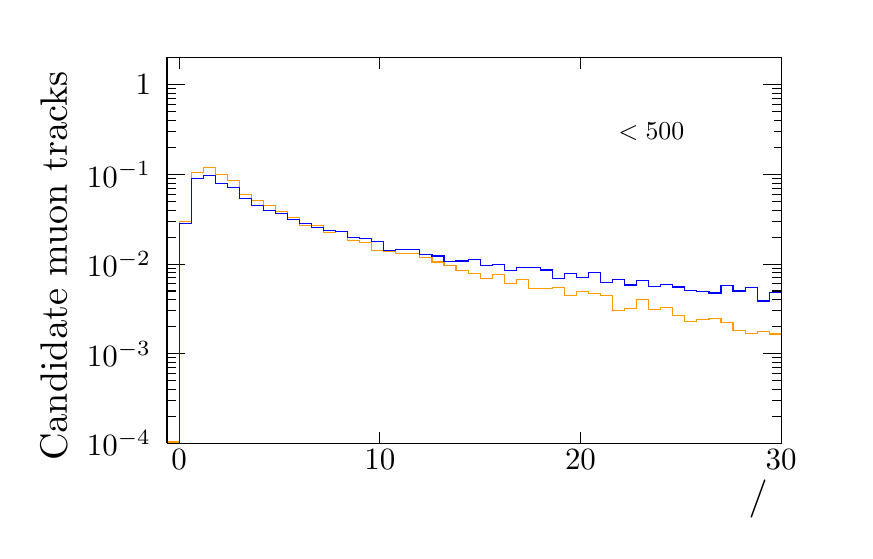
\begin{tikzpicture}
\pgfdeclareplotmark{cross} {
\pgfpathmoveto{\pgfpoint{-0.3\pgfplotmarksize}{\pgfplotmarksize}}
\pgfpathlineto{\pgfpoint{+0.3\pgfplotmarksize}{\pgfplotmarksize}}
\pgfpathlineto{\pgfpoint{+0.3\pgfplotmarksize}{0.3\pgfplotmarksize}}
\pgfpathlineto{\pgfpoint{+1\pgfplotmarksize}{0.3\pgfplotmarksize}}
\pgfpathlineto{\pgfpoint{+1\pgfplotmarksize}{-0.3\pgfplotmarksize}}
\pgfpathlineto{\pgfpoint{+0.3\pgfplotmarksize}{-0.3\pgfplotmarksize}}
\pgfpathlineto{\pgfpoint{+0.3\pgfplotmarksize}{-1.\pgfplotmarksize}}
\pgfpathlineto{\pgfpoint{-0.3\pgfplotmarksize}{-1.\pgfplotmarksize}}
\pgfpathlineto{\pgfpoint{-0.3\pgfplotmarksize}{-0.3\pgfplotmarksize}}
\pgfpathlineto{\pgfpoint{-1.\pgfplotmarksize}{-0.3\pgfplotmarksize}}
\pgfpathlineto{\pgfpoint{-1.\pgfplotmarksize}{0.3\pgfplotmarksize}}
\pgfpathlineto{\pgfpoint{-0.3\pgfplotmarksize}{0.3\pgfplotmarksize}}
\pgfpathclose
\pgfusepathqstroke
}
\pgfdeclareplotmark{cross*} {
\pgfpathmoveto{\pgfpoint{-0.3\pgfplotmarksize}{\pgfplotmarksize}}
\pgfpathlineto{\pgfpoint{+0.3\pgfplotmarksize}{\pgfplotmarksize}}
\pgfpathlineto{\pgfpoint{+0.3\pgfplotmarksize}{0.3\pgfplotmarksize}}
\pgfpathlineto{\pgfpoint{+1\pgfplotmarksize}{0.3\pgfplotmarksize}}
\pgfpathlineto{\pgfpoint{+1\pgfplotmarksize}{-0.3\pgfplotmarksize}}
\pgfpathlineto{\pgfpoint{+0.3\pgfplotmarksize}{-0.3\pgfplotmarksize}}
\pgfpathlineto{\pgfpoint{+0.3\pgfplotmarksize}{-1.\pgfplotmarksize}}
\pgfpathlineto{\pgfpoint{-0.3\pgfplotmarksize}{-1.\pgfplotmarksize}}
\pgfpathlineto{\pgfpoint{-0.3\pgfplotmarksize}{-0.3\pgfplotmarksize}}
\pgfpathlineto{\pgfpoint{-1.\pgfplotmarksize}{-0.3\pgfplotmarksize}}
\pgfpathlineto{\pgfpoint{-1.\pgfplotmarksize}{0.3\pgfplotmarksize}}
\pgfpathlineto{\pgfpoint{-0.3\pgfplotmarksize}{0.3\pgfplotmarksize}}
\pgfpathclose
\pgfusepathqfillstroke
}
\pgfdeclareplotmark{newstar} {
\pgfpathmoveto{\pgfqpoint{0pt}{\pgfplotmarksize}}
\pgfpathlineto{\pgfqpointpolar{44}{0.5\pgfplotmarksize}}
\pgfpathlineto{\pgfqpointpolar{18}{\pgfplotmarksize}}
\pgfpathlineto{\pgfqpointpolar{-20}{0.5\pgfplotmarksize}}
\pgfpathlineto{\pgfqpointpolar{-54}{\pgfplotmarksize}}
\pgfpathlineto{\pgfqpointpolar{-90}{0.5\pgfplotmarksize}}
\pgfpathlineto{\pgfqpointpolar{234}{\pgfplotmarksize}}
\pgfpathlineto{\pgfqpointpolar{198}{0.5\pgfplotmarksize}}
\pgfpathlineto{\pgfqpointpolar{162}{\pgfplotmarksize}}
\pgfpathlineto{\pgfqpointpolar{134}{0.5\pgfplotmarksize}}
\pgfpathclose
\pgfusepathqstroke
}
\pgfdeclareplotmark{newstar*} {
\pgfpathmoveto{\pgfqpoint{0pt}{\pgfplotmarksize}}
\pgfpathlineto{\pgfqpointpolar{44}{0.5\pgfplotmarksize}}
\pgfpathlineto{\pgfqpointpolar{18}{\pgfplotmarksize}}
\pgfpathlineto{\pgfqpointpolar{-20}{0.5\pgfplotmarksize}}
\pgfpathlineto{\pgfqpointpolar{-54}{\pgfplotmarksize}}
\pgfpathlineto{\pgfqpointpolar{-90}{0.5\pgfplotmarksize}}
\pgfpathlineto{\pgfqpointpolar{234}{\pgfplotmarksize}}
\pgfpathlineto{\pgfqpointpolar{198}{0.5\pgfplotmarksize}}
\pgfpathlineto{\pgfqpointpolar{162}{\pgfplotmarksize}}
\pgfpathlineto{\pgfqpointpolar{134}{0.5\pgfplotmarksize}}
\pgfpathclose
\pgfusepathqfillstroke
}
\definecolor{c}{rgb}{1,1,1};
\draw [color=c, fill=c] (0,0) rectangle (10,6.27517);
\draw [color=c, fill=c] (1.4,1.00403) rectangle (9.2,5.89866);
\definecolor{c}{rgb}{0,0,0};
\draw [c] (1.4,1.00403) -- (1.4,5.89866) -- (9.2,5.89866) -- (9.2,1.00403) -- (1.4,1.00403);
\definecolor{c}{rgb}{1,1,1};
\draw [color=c, fill=c] (1.4,1.00403) rectangle (9.2,5.89866);
\definecolor{c}{rgb}{0,0,0};
\draw [c] (1.4,1.00403) -- (1.4,5.89866) -- (9.2,5.89866) -- (9.2,1.00403) -- (1.4,1.00403);
\definecolor{c}{rgb}{1,0.6,0};
\draw [c,line width=0.4] (1.41678,1.02081) -- (1.41678,1.02081) -- (1.55294,1.02081) -- (1.55294,3.82277) -- (1.70588,3.82277) -- (1.70588,4.43859) -- (1.85882,4.43859) -- (1.85882,4.50284) -- (2.01176,4.50284) -- (2.01176,4.41416) --
 (2.16471,4.41416) -- (2.16471,4.3398) -- (2.31765,4.3398) -- (2.31765,4.16077) -- (2.47059,4.16077) -- (2.47059,4.08455) -- (2.62353,4.08455) -- (2.62353,4.0208) -- (2.77647,4.0208) -- (2.77647,3.95189) -- (2.92941,3.95189) -- (2.92941,3.8718) --
 (3.08235,3.8718) -- (3.08235,3.77058) -- (3.23529,3.77058) -- (3.23529,3.77338) -- (3.38824,3.77338) -- (3.38824,3.68092) -- (3.54118,3.68092) -- (3.54118,3.68894) -- (3.69412,3.68894) -- (3.69412,3.57799) -- (3.84706,3.57799) -- (3.84706,3.55246)
 -- (4,3.55246) -- (4,3.45638) -- (4.15294,3.45638) -- (4.15294,3.44021) -- (4.30588,3.44021) -- (4.30588,3.41202) -- (4.45882,3.41202) -- (4.45882,3.41086) -- (4.61176,3.41086) -- (4.61176,3.36201) -- (4.76471,3.36201) -- (4.76471,3.30636) --
 (4.91765,3.30636) -- (4.91765,3.26126) -- (5.07059,3.26126) -- (5.07059,3.19751) -- (5.22353,3.19751) -- (5.22353,3.16418) -- (5.37647,3.16418) -- (5.37647,3.09212) -- (5.52941,3.09212) -- (5.52941,3.14861) -- (5.68235,3.14861) -- (5.68235,3.02834)
 -- (5.83529,3.02834) -- (5.83529,3.08318) -- (5.98824,3.08318) -- (5.98824,2.97233) -- (6.14118,2.97233) -- (6.14118,2.96665) -- (6.29412,2.96665) -- (6.29412,2.98073) -- (6.44706,2.98073) -- (6.44706,2.88616) -- (6.6,2.88616) -- (6.6,2.93722) --
 (6.75294,2.93722) -- (6.75294,2.90269) -- (6.90588,2.90269) -- (6.90588,2.88278) -- (7.05882,2.88278) -- (7.05882,2.69575) -- (7.21176,2.69575) -- (7.21176,2.71986) -- (7.36471,2.71986) -- (7.36471,2.8292) -- (7.51765,2.8292) -- (7.51765,2.70067) --
 (7.67059,2.70067) -- (7.67059,2.72919) -- (7.82353,2.72919) -- (7.82353,2.62692) -- (7.97647,2.62692) -- (7.97647,2.55357) -- (8.12941,2.55357) -- (8.12941,2.57925) -- (8.28235,2.57925) -- (8.28235,2.58546) -- (8.43529,2.58546) -- (8.43529,2.54021)
 -- (8.58823,2.54021) -- (8.58823,2.43497) -- (8.74118,2.43497) -- (8.74118,2.40028) -- (8.89412,2.40028) -- (8.89412,2.42653) -- (9.04706,2.42653) -- (9.04706,2.39121) -- (9.2,2.39121) -- (9.2,1.02081);
\definecolor{c}{rgb}{0,0,0};
\draw [c,line width=0.4] (1.4,1.00403) -- (9.2,1.00403);
\draw [anchor= east] (9.2,0.301208) node[scale=1.37879, rotate=0]{$\chisq/\nDoF$};
\draw [c,line width=0.4] (1.55294,1.15087) -- (1.55294,1.00403);
\draw [c,line width=0.4] (4.10196,1.15087) -- (4.10196,1.00403);
\draw [c,line width=0.4] (6.65098,1.15087) -- (6.65098,1.00403);
\draw [c,line width=0.4] (9.2,1.15087) -- (9.2,1.00403);
\draw [c,line width=0.4] (1.55294,1.15087) -- (1.55294,1.00403);
\draw [anchor=base] (1.55294,0.665168) node[scale=1.11794, rotate=0]{0};
\draw [anchor=base] (4.10196,0.665168) node[scale=1.11794, rotate=0]{10};
\draw [anchor=base] (6.65098,0.665168) node[scale=1.11794, rotate=0]{20};
\draw [anchor=base] (9.2,0.665168) node[scale=1.11794, rotate=0]{30};
\draw [c,line width=0.4] (1.4,5.89866) -- (9.2,5.89866);
\draw [c,line width=0.4] (1.55294,5.75182) -- (1.55294,5.89866);
\draw [c,line width=0.4] (4.10196,5.75182) -- (4.10196,5.89866);
\draw [c,line width=0.4] (6.65098,5.75182) -- (6.65098,5.89866);
\draw [c,line width=0.4] (9.2,5.75182) -- (9.2,5.89866);
\draw [c,line width=0.4] (1.55294,5.75182) -- (1.55294,5.89866);
\draw [c,line width=0.4] (1.4,1.00403) -- (1.4,5.89866);
\draw [anchor= east] (-0.04,5.89866) node[scale=1.37879, rotate=90]{Candidate muon tracks};
\draw [c,line width=0.4] (1.634,1.00403) -- (1.4,1.00403);
\draw [anchor= east] (1.336,1.00403) node[scale=1.11794, rotate=0]{$10^{-4}$};
\draw [c,line width=0.4] (1.517,1.3466) -- (1.4,1.3466);
\draw [c,line width=0.4] (1.517,1.547) -- (1.4,1.547);
\draw [c,line width=0.4] (1.517,1.68918) -- (1.4,1.68918);
\draw [c,line width=0.4] (1.517,1.79947) -- (1.4,1.79947);
\draw [c,line width=0.4] (1.517,1.88957) -- (1.4,1.88957);
\draw [c,line width=0.4] (1.517,1.96576) -- (1.4,1.96576);
\draw [c,line width=0.4] (1.517,2.03176) -- (1.4,2.03176);
\draw [c,line width=0.4] (1.517,2.08997) -- (1.4,2.08997);
\draw [c,line width=0.4] (1.634,2.14204) -- (1.4,2.14204);
\draw [anchor= east] (1.336,2.14204) node[scale=1.11794, rotate=0]{$10^{-3}$};
\draw [c,line width=0.4] (1.517,2.48462) -- (1.4,2.48462);
\draw [c,line width=0.4] (1.517,2.68501) -- (1.4,2.68501);
\draw [c,line width=0.4] (1.517,2.82719) -- (1.4,2.82719);
\draw [c,line width=0.4] (1.517,2.93748) -- (1.4,2.93748);
\draw [c,line width=0.4] (1.517,3.02759) -- (1.4,3.02759);
\draw [c,line width=0.4] (1.517,3.10377) -- (1.4,3.10377);
\draw [c,line width=0.4] (1.517,3.16977) -- (1.4,3.16977);
\draw [c,line width=0.4] (1.517,3.22798) -- (1.4,3.22798);
\draw [c,line width=0.4] (1.634,3.28005) -- (1.4,3.28005);
\draw [anchor= east] (1.336,3.28005) node[scale=1.11794, rotate=0]{$10^{-2}$};
\draw [c,line width=0.4] (1.517,3.62263) -- (1.4,3.62263);
\draw [c,line width=0.4] (1.517,3.82303) -- (1.4,3.82303);
\draw [c,line width=0.4] (1.517,3.96521) -- (1.4,3.96521);
\draw [c,line width=0.4] (1.517,4.07549) -- (1.4,4.07549);
\draw [c,line width=0.4] (1.517,4.1656) -- (1.4,4.1656);
\draw [c,line width=0.4] (1.517,4.24179) -- (1.4,4.24179);
\draw [c,line width=0.4] (1.517,4.30778) -- (1.4,4.30778);
\draw [c,line width=0.4] (1.517,4.366) -- (1.4,4.366);
\draw [c,line width=0.4] (1.634,4.41807) -- (1.4,4.41807);
\draw [anchor= east] (1.336,4.41807) node[scale=1.11794, rotate=0]{$10^{-1}$};
\draw [c,line width=0.4] (1.517,4.76064) -- (1.4,4.76064);
\draw [c,line width=0.4] (1.517,4.96104) -- (1.4,4.96104);
\draw [c,line width=0.4] (1.517,5.10322) -- (1.4,5.10322);
\draw [c,line width=0.4] (1.517,5.21351) -- (1.4,5.21351);
\draw [c,line width=0.4] (1.517,5.30361) -- (1.4,5.30361);
\draw [c,line width=0.4] (1.517,5.3798) -- (1.4,5.3798);
\draw [c,line width=0.4] (1.517,5.4458) -- (1.4,5.4458);
\draw [c,line width=0.4] (1.517,5.50401) -- (1.4,5.50401);
\draw [c,line width=0.4] (1.634,5.55608) -- (1.4,5.55608);
\draw [anchor= east] (1.336,5.55608) node[scale=1.11794, rotate=0]{1};
\draw [c,line width=0.4] (1.517,5.89866) -- (1.4,5.89866);
\draw [c,line width=0.4] (9.2,1.00403) -- (9.2,5.89866);
\draw [c,line width=0.4] (8.966,1.00403) -- (9.2,1.00403);
\draw [c,line width=0.4] (9.083,1.3466) -- (9.2,1.3466);
\draw [c,line width=0.4] (9.083,1.547) -- (9.2,1.547);
\draw [c,line width=0.4] (9.083,1.68918) -- (9.2,1.68918);
\draw [c,line width=0.4] (9.083,1.79947) -- (9.2,1.79947);
\draw [c,line width=0.4] (9.083,1.88957) -- (9.2,1.88957);
\draw [c,line width=0.4] (9.083,1.96576) -- (9.2,1.96576);
\draw [c,line width=0.4] (9.083,2.03176) -- (9.2,2.03176);
\draw [c,line width=0.4] (9.083,2.08997) -- (9.2,2.08997);
\draw [c,line width=0.4] (8.966,2.14204) -- (9.2,2.14204);
\draw [c,line width=0.4] (9.083,2.48462) -- (9.2,2.48462);
\draw [c,line width=0.4] (9.083,2.68501) -- (9.2,2.68501);
\draw [c,line width=0.4] (9.083,2.82719) -- (9.2,2.82719);
\draw [c,line width=0.4] (9.083,2.93748) -- (9.2,2.93748);
\draw [c,line width=0.4] (9.083,3.02759) -- (9.2,3.02759);
\draw [c,line width=0.4] (9.083,3.10377) -- (9.2,3.10377);
\draw [c,line width=0.4] (9.083,3.16977) -- (9.2,3.16977);
\draw [c,line width=0.4] (9.083,3.22798) -- (9.2,3.22798);
\draw [c,line width=0.4] (8.966,3.28005) -- (9.2,3.28005);
\draw [c,line width=0.4] (9.083,3.62263) -- (9.2,3.62263);
\draw [c,line width=0.4] (9.083,3.82303) -- (9.2,3.82303);
\draw [c,line width=0.4] (9.083,3.96521) -- (9.2,3.96521);
\draw [c,line width=0.4] (9.083,4.07549) -- (9.2,4.07549);
\draw [c,line width=0.4] (9.083,4.1656) -- (9.2,4.1656);
\draw [c,line width=0.4] (9.083,4.24179) -- (9.2,4.24179);
\draw [c,line width=0.4] (9.083,4.30778) -- (9.2,4.30778);
\draw [c,line width=0.4] (9.083,4.366) -- (9.2,4.366);
\draw [c,line width=0.4] (8.966,4.41807) -- (9.2,4.41807);
\draw [c,line width=0.4] (9.083,4.76064) -- (9.2,4.76064);
\draw [c,line width=0.4] (9.083,4.96104) -- (9.2,4.96104);
\draw [c,line width=0.4] (9.083,5.10322) -- (9.2,5.10322);
\draw [c,line width=0.4] (9.083,5.21351) -- (9.2,5.21351);
\draw [c,line width=0.4] (9.083,5.30361) -- (9.2,5.30361);
\draw [c,line width=0.4] (9.083,5.3798) -- (9.2,5.3798);
\draw [c,line width=0.4] (9.083,5.4458) -- (9.2,5.4458);
\draw [c,line width=0.4] (9.083,5.50401) -- (9.2,5.50401);
\draw [c,line width=0.4] (8.966,5.55608) -- (9.2,5.55608);
\draw [c,line width=0.4] (9.083,5.89866) -- (9.2,5.89866);
\definecolor{c}{rgb}{0,0,1};
\draw [c,line width=0.4] (1.55294,1.02081) -- (1.55294,3.79674) -- (1.70588,3.79674) -- (1.70588,4.36712) -- (1.85882,4.36712) -- (1.85882,4.40799) -- (2.01176,4.40799) -- (2.01176,4.30465) -- (2.16471,4.30465) -- (2.16471,4.2558) -- (2.31765,4.2558)
 -- (2.31765,4.11481) -- (2.47059,4.11481) -- (2.47059,4.01966) -- (2.62353,4.01966) -- (2.62353,3.96151) -- (2.77647,3.96151) -- (2.77647,3.92204) -- (2.92941,3.92204) -- (2.92941,3.84845) -- (3.08235,3.84845) -- (3.08235,3.78957) --
 (3.23529,3.78957) -- (3.23529,3.74471) -- (3.38824,3.74471) -- (3.38824,3.70354) -- (3.54118,3.70354) -- (3.54118,3.69922) -- (3.69412,3.69922) -- (3.69412,3.62063) -- (3.84706,3.62063) -- (3.84706,3.59989) -- (4,3.59989) -- (4,3.56389) --
 (4.15294,3.56389) -- (4.15294,3.4474) -- (4.30588,3.4474) -- (4.30588,3.46857) -- (4.45882,3.46857) -- (4.45882,3.46083) -- (4.61176,3.46083) -- (4.61176,3.39595) -- (4.76471,3.39595) -- (4.76471,3.38243) -- (4.91765,3.38243) -- (4.91765,3.31604) --
 (5.07059,3.31604) -- (5.07059,3.31917) -- (5.22353,3.31917) -- (5.22353,3.33249) -- (5.37647,3.33249) -- (5.37647,3.25966) -- (5.52941,3.25966) -- (5.52941,3.27918) -- (5.68235,3.27918) -- (5.68235,3.19998) -- (5.83529,3.19998) -- (5.83529,3.23566)
 -- (5.98824,3.23566) -- (5.98824,3.23072) -- (6.14118,3.23072) -- (6.14118,3.20524) -- (6.29412,3.20524) -- (6.29412,3.09918) -- (6.44706,3.09918) -- (6.44706,3.16295) -- (6.6,3.16295) -- (6.6,3.11356) -- (6.75294,3.11356) -- (6.75294,3.17282) --
 (6.90588,3.17282) -- (6.90588,3.0444) -- (7.05882,3.0444) -- (7.05882,3.08438) -- (7.21176,3.08438) -- (7.21176,3.01455) -- (7.36471,3.01455) -- (7.36471,3.06912) -- (7.51765,3.06912) -- (7.51765,2.99892) -- (7.67059,2.99892) -- (7.67059,3.01647) --
 (7.82353,3.01647) -- (7.82353,2.9889) -- (7.97647,2.9889) -- (7.97647,2.94663) -- (8.12941,2.94663) -- (8.12941,2.93094) -- (8.28235,2.93094) -- (8.28235,2.91237) -- (8.43529,2.91237) -- (8.43529,3.01069) -- (8.58823,3.01069) -- (8.58823,2.93773) --
 (8.74118,2.93773) -- (8.74118,2.98483) -- (8.89412,2.98483) -- (8.89412,2.8103) -- (9.04706,2.8103) -- (9.04706,2.92174) -- (9.2,2.92174);
\definecolor{c}{rgb}{1,1,1};
\draw [color=c, fill=c] (6,4.70638) rectangle (9.1,5.20839);
\draw (7.55,4.95738) node[scale=0.931615, rotate=0]{$\pt < 500 \mevc$};
\end{tikzpicture}
}
    \caption{}
    \label{mvTTm_chi2}
  \end{subfigure}%
  \hfill%
  \begin{subfigure}{0.5\textwidth}
    \tikzsetnextfilename{mvTTm_chi2_sigpt_smaller}
    \scalebox{.6}{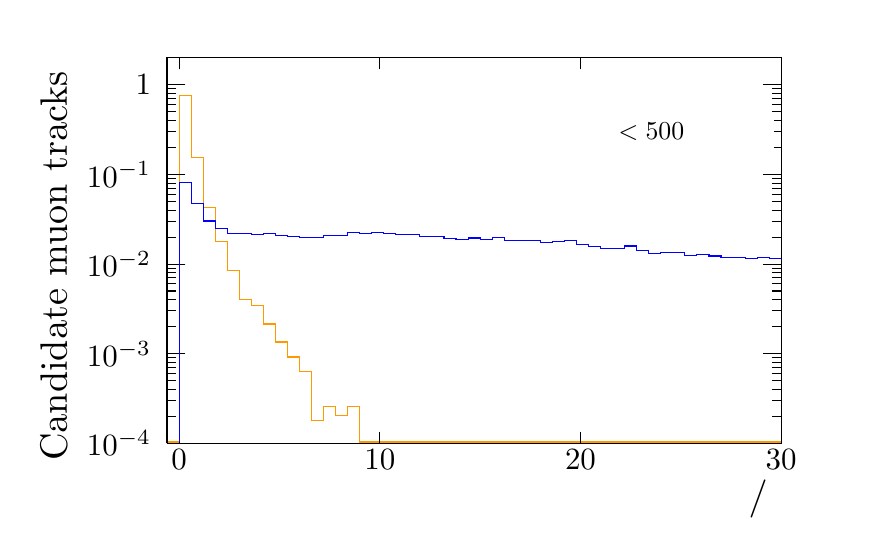
\begin{tikzpicture}
\pgfdeclareplotmark{cross} {
\pgfpathmoveto{\pgfpoint{-0.3\pgfplotmarksize}{\pgfplotmarksize}}
\pgfpathlineto{\pgfpoint{+0.3\pgfplotmarksize}{\pgfplotmarksize}}
\pgfpathlineto{\pgfpoint{+0.3\pgfplotmarksize}{0.3\pgfplotmarksize}}
\pgfpathlineto{\pgfpoint{+1\pgfplotmarksize}{0.3\pgfplotmarksize}}
\pgfpathlineto{\pgfpoint{+1\pgfplotmarksize}{-0.3\pgfplotmarksize}}
\pgfpathlineto{\pgfpoint{+0.3\pgfplotmarksize}{-0.3\pgfplotmarksize}}
\pgfpathlineto{\pgfpoint{+0.3\pgfplotmarksize}{-1.\pgfplotmarksize}}
\pgfpathlineto{\pgfpoint{-0.3\pgfplotmarksize}{-1.\pgfplotmarksize}}
\pgfpathlineto{\pgfpoint{-0.3\pgfplotmarksize}{-0.3\pgfplotmarksize}}
\pgfpathlineto{\pgfpoint{-1.\pgfplotmarksize}{-0.3\pgfplotmarksize}}
\pgfpathlineto{\pgfpoint{-1.\pgfplotmarksize}{0.3\pgfplotmarksize}}
\pgfpathlineto{\pgfpoint{-0.3\pgfplotmarksize}{0.3\pgfplotmarksize}}
\pgfpathclose
\pgfusepathqstroke
}
\pgfdeclareplotmark{cross*} {
\pgfpathmoveto{\pgfpoint{-0.3\pgfplotmarksize}{\pgfplotmarksize}}
\pgfpathlineto{\pgfpoint{+0.3\pgfplotmarksize}{\pgfplotmarksize}}
\pgfpathlineto{\pgfpoint{+0.3\pgfplotmarksize}{0.3\pgfplotmarksize}}
\pgfpathlineto{\pgfpoint{+1\pgfplotmarksize}{0.3\pgfplotmarksize}}
\pgfpathlineto{\pgfpoint{+1\pgfplotmarksize}{-0.3\pgfplotmarksize}}
\pgfpathlineto{\pgfpoint{+0.3\pgfplotmarksize}{-0.3\pgfplotmarksize}}
\pgfpathlineto{\pgfpoint{+0.3\pgfplotmarksize}{-1.\pgfplotmarksize}}
\pgfpathlineto{\pgfpoint{-0.3\pgfplotmarksize}{-1.\pgfplotmarksize}}
\pgfpathlineto{\pgfpoint{-0.3\pgfplotmarksize}{-0.3\pgfplotmarksize}}
\pgfpathlineto{\pgfpoint{-1.\pgfplotmarksize}{-0.3\pgfplotmarksize}}
\pgfpathlineto{\pgfpoint{-1.\pgfplotmarksize}{0.3\pgfplotmarksize}}
\pgfpathlineto{\pgfpoint{-0.3\pgfplotmarksize}{0.3\pgfplotmarksize}}
\pgfpathclose
\pgfusepathqfillstroke
}
\pgfdeclareplotmark{newstar} {
\pgfpathmoveto{\pgfqpoint{0pt}{\pgfplotmarksize}}
\pgfpathlineto{\pgfqpointpolar{44}{0.5\pgfplotmarksize}}
\pgfpathlineto{\pgfqpointpolar{18}{\pgfplotmarksize}}
\pgfpathlineto{\pgfqpointpolar{-20}{0.5\pgfplotmarksize}}
\pgfpathlineto{\pgfqpointpolar{-54}{\pgfplotmarksize}}
\pgfpathlineto{\pgfqpointpolar{-90}{0.5\pgfplotmarksize}}
\pgfpathlineto{\pgfqpointpolar{234}{\pgfplotmarksize}}
\pgfpathlineto{\pgfqpointpolar{198}{0.5\pgfplotmarksize}}
\pgfpathlineto{\pgfqpointpolar{162}{\pgfplotmarksize}}
\pgfpathlineto{\pgfqpointpolar{134}{0.5\pgfplotmarksize}}
\pgfpathclose
\pgfusepathqstroke
}
\pgfdeclareplotmark{newstar*} {
\pgfpathmoveto{\pgfqpoint{0pt}{\pgfplotmarksize}}
\pgfpathlineto{\pgfqpointpolar{44}{0.5\pgfplotmarksize}}
\pgfpathlineto{\pgfqpointpolar{18}{\pgfplotmarksize}}
\pgfpathlineto{\pgfqpointpolar{-20}{0.5\pgfplotmarksize}}
\pgfpathlineto{\pgfqpointpolar{-54}{\pgfplotmarksize}}
\pgfpathlineto{\pgfqpointpolar{-90}{0.5\pgfplotmarksize}}
\pgfpathlineto{\pgfqpointpolar{234}{\pgfplotmarksize}}
\pgfpathlineto{\pgfqpointpolar{198}{0.5\pgfplotmarksize}}
\pgfpathlineto{\pgfqpointpolar{162}{\pgfplotmarksize}}
\pgfpathlineto{\pgfqpointpolar{134}{0.5\pgfplotmarksize}}
\pgfpathclose
\pgfusepathqfillstroke
}
\definecolor{c}{rgb}{1,1,1};
\draw [color=c, fill=c] (0,0) rectangle (10,6.27517);
\draw [color=c, fill=c] (1.4,1.00403) rectangle (9.2,5.89866);
\definecolor{c}{rgb}{0,0,0};
\draw [c] (1.4,1.00403) -- (1.4,5.89866) -- (9.2,5.89866) -- (9.2,1.00403) -- (1.4,1.00403);
\definecolor{c}{rgb}{1,1,1};
\draw [color=c, fill=c] (1.4,1.00403) rectangle (9.2,5.89866);
\definecolor{c}{rgb}{0,0,0};
\draw [c] (1.4,1.00403) -- (1.4,5.89866) -- (9.2,5.89866) -- (9.2,1.00403) -- (1.4,1.00403);
\definecolor{c}{rgb}{1,0.6,0};
\draw [c,line width=0.4] (1.41678,1.02081) -- (1.41678,1.02081) -- (1.55294,1.02081) -- (1.55294,5.42255) -- (1.70588,5.42255) -- (1.70588,4.62973) -- (1.85882,4.62973) -- (1.85882,4.00033) -- (2.01176,4.00033) -- (2.01176,3.56618) --
 (2.16471,3.56618) -- (2.16471,3.20048) -- (2.31765,3.20048) -- (2.31765,2.83364) -- (2.47059,2.83364) -- (2.47059,2.75277) -- (2.62353,2.75277) -- (2.62353,2.51827) -- (2.77647,2.51827) -- (2.77647,2.29067) -- (2.92941,2.29067) -- (2.92941,2.09951)
 -- (3.08235,2.09951) -- (3.08235,1.91929) -- (3.23529,1.91929) -- (3.23529,1.29015) -- (3.38824,1.29015) -- (3.38824,1.46643) -- (3.54118,1.46643) -- (3.54118,1.35615) -- (3.69412,1.35615) -- (3.69412,1.46643) -- (3.84706,1.46643) --
 (3.84706,1.02081) -- (4,1.02081) -- (4,1.02081) -- (4.15294,1.02081) -- (4.15294,1.02081) -- (4.30588,1.02081) -- (4.30588,1.02081) -- (4.45882,1.02081) -- (4.45882,1.02081) -- (4.61176,1.02081) -- (4.61176,1.02081) -- (4.76471,1.02081) --
 (4.76471,1.02081) -- (4.91765,1.02081) -- (4.91765,1.02081) -- (5.07059,1.02081) -- (5.07059,1.02081) -- (5.22353,1.02081) -- (5.22353,1.02081) -- (5.37647,1.02081) -- (5.37647,1.02081) -- (5.52941,1.02081) -- (5.52941,1.02081) -- (5.68235,1.02081)
 -- (5.68235,1.02081) -- (5.83529,1.02081) -- (5.83529,1.02081) -- (5.98824,1.02081) -- (5.98824,1.02081) -- (6.14118,1.02081) -- (6.14118,1.02081) -- (6.29412,1.02081) -- (6.29412,1.02081) -- (6.44706,1.02081) -- (6.44706,1.02081) -- (6.6,1.02081)
 -- (6.6,1.02081) -- (6.75294,1.02081) -- (6.75294,1.02081) -- (6.90588,1.02081) -- (6.90588,1.02081) -- (7.05882,1.02081) -- (7.05882,1.02081) -- (7.21176,1.02081) -- (7.21176,1.02081) -- (7.36471,1.02081) -- (7.36471,1.02081) -- (7.51765,1.02081)
 -- (7.51765,1.02081) -- (7.67059,1.02081) -- (7.67059,1.02081) -- (7.82353,1.02081) -- (7.82353,1.02081) -- (7.97647,1.02081) -- (7.97647,1.02081) -- (8.12941,1.02081) -- (8.12941,1.02081) -- (8.28235,1.02081) -- (8.28235,1.02081) --
 (8.43529,1.02081) -- (8.43529,1.02081) -- (8.58823,1.02081) -- (8.58823,1.02081) -- (8.74118,1.02081) -- (8.74118,1.02081) -- (8.89412,1.02081) -- (8.89412,1.02081) -- (9.04706,1.02081) -- (9.04706,1.02081) -- (9.2,1.02081) -- (9.2,1.02081);
\definecolor{c}{rgb}{0,0,0};
\draw [c,line width=0.4] (1.4,1.00403) -- (9.2,1.00403);
\draw [anchor= east] (9.2,0.301208) node[scale=1.37879, rotate=0]{$\chisq/\nDoF$};
\draw [c,line width=0.4] (1.55294,1.15087) -- (1.55294,1.00403);
\draw [c,line width=0.4] (4.10196,1.15087) -- (4.10196,1.00403);
\draw [c,line width=0.4] (6.65098,1.15087) -- (6.65098,1.00403);
\draw [c,line width=0.4] (9.2,1.15087) -- (9.2,1.00403);
\draw [c,line width=0.4] (1.55294,1.15087) -- (1.55294,1.00403);
\draw [anchor=base] (1.55294,0.665168) node[scale=1.11794, rotate=0]{0};
\draw [anchor=base] (4.10196,0.665168) node[scale=1.11794, rotate=0]{10};
\draw [anchor=base] (6.65098,0.665168) node[scale=1.11794, rotate=0]{20};
\draw [anchor=base] (9.2,0.665168) node[scale=1.11794, rotate=0]{30};
\draw [c,line width=0.4] (1.4,5.89866) -- (9.2,5.89866);
\draw [c,line width=0.4] (1.55294,5.75182) -- (1.55294,5.89866);
\draw [c,line width=0.4] (4.10196,5.75182) -- (4.10196,5.89866);
\draw [c,line width=0.4] (6.65098,5.75182) -- (6.65098,5.89866);
\draw [c,line width=0.4] (9.2,5.75182) -- (9.2,5.89866);
\draw [c,line width=0.4] (1.55294,5.75182) -- (1.55294,5.89866);
\draw [c,line width=0.4] (1.4,1.00403) -- (1.4,5.89866);
\draw [anchor= east] (-0.04,5.89866) node[scale=1.37879, rotate=90]{Candidate muon tracks};
\draw [c,line width=0.4] (1.634,1.00403) -- (1.4,1.00403);
\draw [anchor= east] (1.336,1.00403) node[scale=1.11794, rotate=0]{$10^{-4}$};
\draw [c,line width=0.4] (1.517,1.3466) -- (1.4,1.3466);
\draw [c,line width=0.4] (1.517,1.547) -- (1.4,1.547);
\draw [c,line width=0.4] (1.517,1.68918) -- (1.4,1.68918);
\draw [c,line width=0.4] (1.517,1.79947) -- (1.4,1.79947);
\draw [c,line width=0.4] (1.517,1.88957) -- (1.4,1.88957);
\draw [c,line width=0.4] (1.517,1.96576) -- (1.4,1.96576);
\draw [c,line width=0.4] (1.517,2.03176) -- (1.4,2.03176);
\draw [c,line width=0.4] (1.517,2.08997) -- (1.4,2.08997);
\draw [c,line width=0.4] (1.634,2.14204) -- (1.4,2.14204);
\draw [anchor= east] (1.336,2.14204) node[scale=1.11794, rotate=0]{$10^{-3}$};
\draw [c,line width=0.4] (1.517,2.48462) -- (1.4,2.48462);
\draw [c,line width=0.4] (1.517,2.68501) -- (1.4,2.68501);
\draw [c,line width=0.4] (1.517,2.82719) -- (1.4,2.82719);
\draw [c,line width=0.4] (1.517,2.93748) -- (1.4,2.93748);
\draw [c,line width=0.4] (1.517,3.02759) -- (1.4,3.02759);
\draw [c,line width=0.4] (1.517,3.10377) -- (1.4,3.10377);
\draw [c,line width=0.4] (1.517,3.16977) -- (1.4,3.16977);
\draw [c,line width=0.4] (1.517,3.22798) -- (1.4,3.22798);
\draw [c,line width=0.4] (1.634,3.28005) -- (1.4,3.28005);
\draw [anchor= east] (1.336,3.28005) node[scale=1.11794, rotate=0]{$10^{-2}$};
\draw [c,line width=0.4] (1.517,3.62263) -- (1.4,3.62263);
\draw [c,line width=0.4] (1.517,3.82303) -- (1.4,3.82303);
\draw [c,line width=0.4] (1.517,3.96521) -- (1.4,3.96521);
\draw [c,line width=0.4] (1.517,4.07549) -- (1.4,4.07549);
\draw [c,line width=0.4] (1.517,4.1656) -- (1.4,4.1656);
\draw [c,line width=0.4] (1.517,4.24179) -- (1.4,4.24179);
\draw [c,line width=0.4] (1.517,4.30778) -- (1.4,4.30778);
\draw [c,line width=0.4] (1.517,4.366) -- (1.4,4.366);
\draw [c,line width=0.4] (1.634,4.41807) -- (1.4,4.41807);
\draw [anchor= east] (1.336,4.41807) node[scale=1.11794, rotate=0]{$10^{-1}$};
\draw [c,line width=0.4] (1.517,4.76064) -- (1.4,4.76064);
\draw [c,line width=0.4] (1.517,4.96104) -- (1.4,4.96104);
\draw [c,line width=0.4] (1.517,5.10322) -- (1.4,5.10322);
\draw [c,line width=0.4] (1.517,5.21351) -- (1.4,5.21351);
\draw [c,line width=0.4] (1.517,5.30361) -- (1.4,5.30361);
\draw [c,line width=0.4] (1.517,5.3798) -- (1.4,5.3798);
\draw [c,line width=0.4] (1.517,5.4458) -- (1.4,5.4458);
\draw [c,line width=0.4] (1.517,5.50401) -- (1.4,5.50401);
\draw [c,line width=0.4] (1.634,5.55608) -- (1.4,5.55608);
\draw [anchor= east] (1.336,5.55608) node[scale=1.11794, rotate=0]{1};
\draw [c,line width=0.4] (1.517,5.89866) -- (1.4,5.89866);
\draw [c,line width=0.4] (9.2,1.00403) -- (9.2,5.89866);
\draw [c,line width=0.4] (8.966,1.00403) -- (9.2,1.00403);
\draw [c,line width=0.4] (9.083,1.3466) -- (9.2,1.3466);
\draw [c,line width=0.4] (9.083,1.547) -- (9.2,1.547);
\draw [c,line width=0.4] (9.083,1.68918) -- (9.2,1.68918);
\draw [c,line width=0.4] (9.083,1.79947) -- (9.2,1.79947);
\draw [c,line width=0.4] (9.083,1.88957) -- (9.2,1.88957);
\draw [c,line width=0.4] (9.083,1.96576) -- (9.2,1.96576);
\draw [c,line width=0.4] (9.083,2.03176) -- (9.2,2.03176);
\draw [c,line width=0.4] (9.083,2.08997) -- (9.2,2.08997);
\draw [c,line width=0.4] (8.966,2.14204) -- (9.2,2.14204);
\draw [c,line width=0.4] (9.083,2.48462) -- (9.2,2.48462);
\draw [c,line width=0.4] (9.083,2.68501) -- (9.2,2.68501);
\draw [c,line width=0.4] (9.083,2.82719) -- (9.2,2.82719);
\draw [c,line width=0.4] (9.083,2.93748) -- (9.2,2.93748);
\draw [c,line width=0.4] (9.083,3.02759) -- (9.2,3.02759);
\draw [c,line width=0.4] (9.083,3.10377) -- (9.2,3.10377);
\draw [c,line width=0.4] (9.083,3.16977) -- (9.2,3.16977);
\draw [c,line width=0.4] (9.083,3.22798) -- (9.2,3.22798);
\draw [c,line width=0.4] (8.966,3.28005) -- (9.2,3.28005);
\draw [c,line width=0.4] (9.083,3.62263) -- (9.2,3.62263);
\draw [c,line width=0.4] (9.083,3.82303) -- (9.2,3.82303);
\draw [c,line width=0.4] (9.083,3.96521) -- (9.2,3.96521);
\draw [c,line width=0.4] (9.083,4.07549) -- (9.2,4.07549);
\draw [c,line width=0.4] (9.083,4.1656) -- (9.2,4.1656);
\draw [c,line width=0.4] (9.083,4.24179) -- (9.2,4.24179);
\draw [c,line width=0.4] (9.083,4.30778) -- (9.2,4.30778);
\draw [c,line width=0.4] (9.083,4.366) -- (9.2,4.366);
\draw [c,line width=0.4] (8.966,4.41807) -- (9.2,4.41807);
\draw [c,line width=0.4] (9.083,4.76064) -- (9.2,4.76064);
\draw [c,line width=0.4] (9.083,4.96104) -- (9.2,4.96104);
\draw [c,line width=0.4] (9.083,5.10322) -- (9.2,5.10322);
\draw [c,line width=0.4] (9.083,5.21351) -- (9.2,5.21351);
\draw [c,line width=0.4] (9.083,5.30361) -- (9.2,5.30361);
\draw [c,line width=0.4] (9.083,5.3798) -- (9.2,5.3798);
\draw [c,line width=0.4] (9.083,5.4458) -- (9.2,5.4458);
\draw [c,line width=0.4] (9.083,5.50401) -- (9.2,5.50401);
\draw [c,line width=0.4] (8.966,5.55608) -- (9.2,5.55608);
\draw [c,line width=0.4] (9.083,5.89866) -- (9.2,5.89866);
\definecolor{c}{rgb}{0,0,1};
\draw [c,line width=0.4] (1.55294,1.02081) -- (1.55294,4.31946) -- (1.70588,4.31946) -- (1.70588,4.04993) -- (1.85882,4.04993) -- (1.85882,3.82753) -- (2.01176,3.82753) -- (2.01176,3.73489) -- (2.16471,3.73489) -- (2.16471,3.6723) -- (2.31765,3.6723)
 -- (2.31765,3.66634) -- (2.47059,3.66634) -- (2.47059,3.65572) -- (2.62353,3.65572) -- (2.62353,3.66634) -- (2.77647,3.66634) -- (2.77647,3.64067) -- (2.92941,3.64067) -- (2.92941,3.63056) -- (3.08235,3.63056) -- (3.08235,3.61748) --
 (3.23529,3.61748) -- (3.23529,3.61526) -- (3.38824,3.61526) -- (3.38824,3.64434) -- (3.54118,3.64434) -- (3.54118,3.64747) -- (3.69412,3.64747) -- (3.69412,3.68451) -- (3.84706,3.68451) -- (3.84706,3.6723) -- (4,3.6723) -- (4,3.68451) --
 (4.15294,3.68451) -- (4.15294,3.6723) -- (4.30588,3.6723) -- (4.30588,3.65979) -- (4.45882,3.65979) -- (4.45882,3.65006) -- (4.61176,3.65006) -- (4.61176,3.62569) -- (4.76471,3.62569) -- (4.76471,3.62948) -- (4.91765,3.62948) -- (4.91765,3.60631) --
 (5.07059,3.60631) -- (5.07059,3.5943) -- (5.22353,3.5943) -- (5.22353,3.61137) -- (5.37647,3.61137) -- (5.37647,3.58789) -- (5.52941,3.58789) -- (5.52941,3.61526) -- (5.68235,3.61526) -- (5.68235,3.5814) -- (5.83529,3.5814) -- (5.83529,3.5814) --
 (5.98824,3.5814) -- (5.98824,3.57783) -- (6.14118,3.57783) -- (6.14118,3.55014) -- (6.29412,3.55014) -- (6.29412,3.56816) -- (6.44706,3.56816) -- (6.44706,3.57723) -- (6.6,3.57723) -- (6.6,3.53078) -- (6.75294,3.53078) -- (6.75294,3.50788) --
 (6.90588,3.50788) -- (6.90588,3.47732) -- (7.05882,3.47732) -- (7.05882,3.48024) -- (7.21176,3.48024) -- (7.21176,3.50926) -- (7.36471,3.50926) -- (7.36471,3.45251) -- (7.51765,3.45251) -- (7.51765,3.41404) -- (7.67059,3.41404) -- (7.67059,3.42882)
 -- (7.82353,3.42882) -- (7.82353,3.42312) -- (7.97647,3.42312) -- (7.97647,3.38397) -- (8.12941,3.38397) -- (8.12941,3.3988) -- (8.28235,3.3988) -- (8.28235,3.3822) -- (8.43529,3.3822) -- (8.43529,3.36132) -- (8.58823,3.36132) -- (8.58823,3.36317)
 -- (8.74118,3.36317) -- (8.74118,3.35195) -- (8.89412,3.35195) -- (8.89412,3.36501) -- (9.04706,3.36501) -- (9.04706,3.3453) -- (9.2,3.3453);
\definecolor{c}{rgb}{1,1,1};
\draw [color=c, fill=c] (6,4.70638) rectangle (9.1,5.20839);
\draw (7.55,4.95738) node[scale=0.931615, rotate=0]{$\pt < 500 \mevc$};
\end{tikzpicture}
}
    \caption{}
    \label{mvm_chi2}
  \end{subfigure}
  \caption{Distribution of the \chisq variable between the old (left) and the new (right) matching algorithms.
           Only low momentum \veloTracks are considered.}
 \label{mvm_chi2_comp}
\end{figure}

\subsubsection{z focal plane parametrization}
The emperical parametrization of the magnet focal plane $z$ coordinate \cite{blah}, already used in  the old \mvm,
is corrected using simulated data. The correction is a function of the inverse momentum. It is extracted by comparing
a proper extrapolation, that describes the magnetic field, with the kick method. The correction is based on the fact
that a good estimate of the z magnet coordinate is the one that gives a momentum estiamte as close to the one from MC.

For the erros something similar is done but I still need to study it a bit. (this correction was done after i submitted my code.)

\subsubsection{M3 Field of Intereset}
As explained in \secref{sec:muon_matching} the M3 FoI $x$ coordintes are computed assuming a minimum track momentum, and thus maximum deflection,
of $6\gevc$. For a $6\gevc$ muon the deflection caused by the \lhcb magnet is computed using the empirical paramtetrization mentioned in Section blah of \cite{roelThesis}.
Using this techinique makes it possible to estimate the region in M3 that a muon track will arrive at without performing the computation
expensive calculation of its trajectory through the \lhcb magnet, also refered to track {\it extrapolation}. In order to visualise the FoI sizes,
simulated events are used to compute the distance of the true hit in M3 from the middle of the FoI, respectivelly in the $x$ and $y$ planes.
The results are shown in \figref{mvm_res}. The average FoI half-width is $2.7\m$ and $0.4\m$ respectivelly for the $x$ and $y$ planes.
Which imples that most of the times the true hit is inside the FoI. The outliers in the \figref{mvTTm_res_x} in with $|d^{M3}|>3\m$
correspond to cases were the track charge estimate by the \ttracker is wrong. Remember that charge information is used to
look for hits only in the one side of the M3 station. Lastly the y plane is the non-bending plane hence the FoI sizes
are smaller, compared to the ones for the $x$ plane, since only multiple scattering is present in that plane.


\begin{figure}[t]
  \centering
  \begin{subfigure}{0.5\textwidth}
    \tikzsetnextfilename{mvTTm_wind_eff_total_x}
    \scalebox{.6}{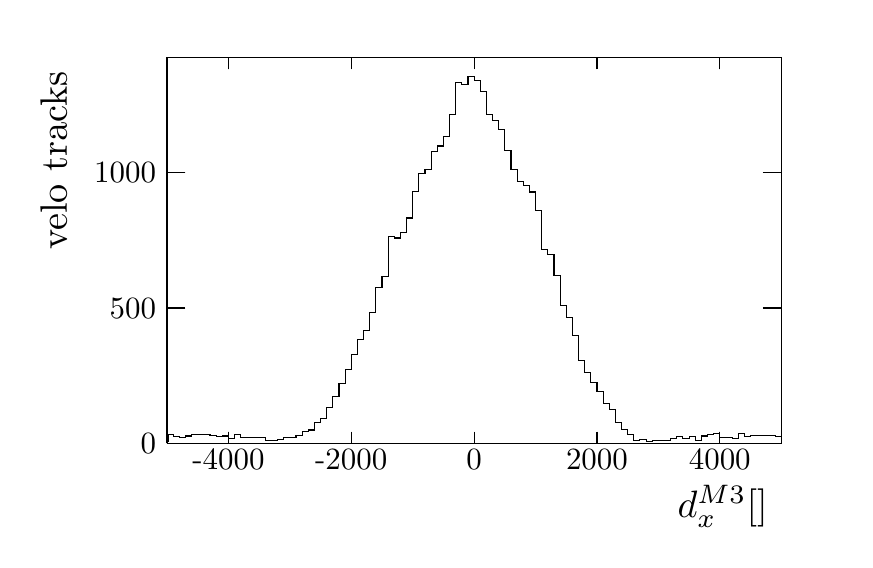
\begin{tikzpicture}
\pgfdeclareplotmark{cross} {
\pgfpathmoveto{\pgfpoint{-0.3\pgfplotmarksize}{\pgfplotmarksize}}
\pgfpathlineto{\pgfpoint{+0.3\pgfplotmarksize}{\pgfplotmarksize}}
\pgfpathlineto{\pgfpoint{+0.3\pgfplotmarksize}{0.3\pgfplotmarksize}}
\pgfpathlineto{\pgfpoint{+1\pgfplotmarksize}{0.3\pgfplotmarksize}}
\pgfpathlineto{\pgfpoint{+1\pgfplotmarksize}{-0.3\pgfplotmarksize}}
\pgfpathlineto{\pgfpoint{+0.3\pgfplotmarksize}{-0.3\pgfplotmarksize}}
\pgfpathlineto{\pgfpoint{+0.3\pgfplotmarksize}{-1.\pgfplotmarksize}}
\pgfpathlineto{\pgfpoint{-0.3\pgfplotmarksize}{-1.\pgfplotmarksize}}
\pgfpathlineto{\pgfpoint{-0.3\pgfplotmarksize}{-0.3\pgfplotmarksize}}
\pgfpathlineto{\pgfpoint{-1.\pgfplotmarksize}{-0.3\pgfplotmarksize}}
\pgfpathlineto{\pgfpoint{-1.\pgfplotmarksize}{0.3\pgfplotmarksize}}
\pgfpathlineto{\pgfpoint{-0.3\pgfplotmarksize}{0.3\pgfplotmarksize}}
\pgfpathclose
\pgfusepathqstroke
}
\pgfdeclareplotmark{cross*} {
\pgfpathmoveto{\pgfpoint{-0.3\pgfplotmarksize}{\pgfplotmarksize}}
\pgfpathlineto{\pgfpoint{+0.3\pgfplotmarksize}{\pgfplotmarksize}}
\pgfpathlineto{\pgfpoint{+0.3\pgfplotmarksize}{0.3\pgfplotmarksize}}
\pgfpathlineto{\pgfpoint{+1\pgfplotmarksize}{0.3\pgfplotmarksize}}
\pgfpathlineto{\pgfpoint{+1\pgfplotmarksize}{-0.3\pgfplotmarksize}}
\pgfpathlineto{\pgfpoint{+0.3\pgfplotmarksize}{-0.3\pgfplotmarksize}}
\pgfpathlineto{\pgfpoint{+0.3\pgfplotmarksize}{-1.\pgfplotmarksize}}
\pgfpathlineto{\pgfpoint{-0.3\pgfplotmarksize}{-1.\pgfplotmarksize}}
\pgfpathlineto{\pgfpoint{-0.3\pgfplotmarksize}{-0.3\pgfplotmarksize}}
\pgfpathlineto{\pgfpoint{-1.\pgfplotmarksize}{-0.3\pgfplotmarksize}}
\pgfpathlineto{\pgfpoint{-1.\pgfplotmarksize}{0.3\pgfplotmarksize}}
\pgfpathlineto{\pgfpoint{-0.3\pgfplotmarksize}{0.3\pgfplotmarksize}}
\pgfpathclose
\pgfusepathqfillstroke
}
\pgfdeclareplotmark{newstar} {
\pgfpathmoveto{\pgfqpoint{0pt}{\pgfplotmarksize}}
\pgfpathlineto{\pgfqpointpolar{44}{0.5\pgfplotmarksize}}
\pgfpathlineto{\pgfqpointpolar{18}{\pgfplotmarksize}}
\pgfpathlineto{\pgfqpointpolar{-20}{0.5\pgfplotmarksize}}
\pgfpathlineto{\pgfqpointpolar{-54}{\pgfplotmarksize}}
\pgfpathlineto{\pgfqpointpolar{-90}{0.5\pgfplotmarksize}}
\pgfpathlineto{\pgfqpointpolar{234}{\pgfplotmarksize}}
\pgfpathlineto{\pgfqpointpolar{198}{0.5\pgfplotmarksize}}
\pgfpathlineto{\pgfqpointpolar{162}{\pgfplotmarksize}}
\pgfpathlineto{\pgfqpointpolar{134}{0.5\pgfplotmarksize}}
\pgfpathclose
\pgfusepathqstroke
}
\pgfdeclareplotmark{newstar*} {
\pgfpathmoveto{\pgfqpoint{0pt}{\pgfplotmarksize}}
\pgfpathlineto{\pgfqpointpolar{44}{0.5\pgfplotmarksize}}
\pgfpathlineto{\pgfqpointpolar{18}{\pgfplotmarksize}}
\pgfpathlineto{\pgfqpointpolar{-20}{0.5\pgfplotmarksize}}
\pgfpathlineto{\pgfqpointpolar{-54}{\pgfplotmarksize}}
\pgfpathlineto{\pgfqpointpolar{-90}{0.5\pgfplotmarksize}}
\pgfpathlineto{\pgfqpointpolar{234}{\pgfplotmarksize}}
\pgfpathlineto{\pgfqpointpolar{198}{0.5\pgfplotmarksize}}
\pgfpathlineto{\pgfqpointpolar{162}{\pgfplotmarksize}}
\pgfpathlineto{\pgfqpointpolar{134}{0.5\pgfplotmarksize}}
\pgfpathclose
\pgfusepathqfillstroke
}
\definecolor{c}{rgb}{1,1,1};
\draw [color=c, fill=c] (0,0) rectangle (10,6.27517);
\draw [color=c, fill=c] (1.4,1.00403) rectangle (9.2,5.89866);
\definecolor{c}{rgb}{0,0,0};
\draw [c] (1.4,1.00403) -- (1.4,5.89866) -- (9.2,5.89866) -- (9.2,1.00403) -- (1.4,1.00403);
\definecolor{c}{rgb}{1,1,1};
\draw [color=c, fill=c] (1.4,1.00403) rectangle (9.2,5.89866);
\definecolor{c}{rgb}{0,0,0};
\draw [c] (1.4,1.00403) -- (1.4,5.89866) -- (9.2,5.89866) -- (9.2,1.00403) -- (1.4,1.00403);
\draw [c,line width=0.4] (1.41678,1.02081) -- (1.41678,1.12082) -- (1.478,1.12082) -- (1.478,1.08647) -- (1.556,1.08647) -- (1.556,1.07617) -- (1.634,1.07617) -- (1.634,1.09678) -- (1.712,1.09678) -- (1.712,1.11395) -- (1.79,1.11395) --
 (1.79,1.11739) -- (1.868,1.11739) -- (1.868,1.11395) -- (1.946,1.11395) -- (1.946,1.10708) -- (2.024,1.10708) -- (2.024,1.09334) -- (2.102,1.09334) -- (2.102,1.09678) -- (2.18,1.09678) -- (2.18,1.0693) -- (2.258,1.0693) -- (2.258,1.11052) --
 (2.336,1.11052) -- (2.336,1.07273) -- (2.414,1.07273) -- (2.414,1.08304) -- (2.492,1.08304) -- (2.492,1.07617) -- (2.57,1.07617) -- (2.57,1.07273) -- (2.648,1.07273) -- (2.648,1.03838) -- (2.726,1.03838) -- (2.726,1.03494) -- (2.804,1.03494) --
 (2.804,1.04868) -- (2.882,1.04868) -- (2.882,1.08304) -- (2.96,1.08304) -- (2.96,1.07617) -- (3.038,1.07617) -- (3.038,1.10708) -- (3.116,1.10708) -- (3.116,1.1483) -- (3.194,1.1483) -- (3.194,1.17235) -- (3.272,1.17235) -- (3.272,1.27197) --
 (3.35,1.27197) -- (3.35,1.31663) -- (3.428,1.31663) -- (3.428,1.45404) -- (3.506,1.45404) -- (3.506,1.59831) -- (3.584,1.59831) -- (3.584,1.76664) -- (3.662,1.76664) -- (3.662,1.94183) -- (3.74,1.94183) -- (3.74,2.1342) -- (3.818,2.1342) --
 (3.818,2.32314) -- (3.896,2.32314) -- (3.896,2.43307) -- (3.974,2.43307) -- (3.974,2.67009) -- (4.052,2.67009) -- (4.052,2.9827) -- (4.13,2.9827) -- (4.13,3.11667) -- (4.208,3.11667) -- (4.208,3.63195) -- (4.286,3.63195) -- (4.286,3.61134) --
 (4.364,3.61134) -- (4.364,3.6766) -- (4.442,3.6766) -- (4.442,3.86554) -- (4.52,3.86554) -- (4.52,4.20562) -- (4.598,4.20562) -- (4.598,4.42891) -- (4.676,4.42891) -- (4.676,4.477) -- (4.754,4.477) -- (4.754,4.7106) -- (4.832,4.7106) --
 (4.832,4.7793) -- (4.91,4.7793) -- (4.91,4.8961) -- (4.988,4.8961) -- (4.988,5.18465) -- (5.066,5.18465) -- (5.066,5.58314) -- (5.144,5.58314) -- (5.144,5.55565) -- (5.222,5.55565) -- (5.222,5.66558) -- (5.3,5.66558) -- (5.3,5.60718) --
 (5.378,5.60718) -- (5.378,5.46977) -- (5.456,5.46977) -- (5.456,5.18465) -- (5.534,5.18465) -- (5.534,5.10221) -- (5.612,5.10221) -- (5.612,4.99228) -- (5.69,4.99228) -- (5.69,4.72777) -- (5.768,4.72777) -- (5.768,4.477) -- (5.846,4.477) --
 (5.846,4.32929) -- (5.924,4.32929) -- (5.924,4.27776) -- (6.002,4.27776) -- (6.002,4.19532) -- (6.08,4.19532) -- (6.08,3.96173) -- (6.158,3.96173) -- (6.158,3.46706) -- (6.236,3.46706) -- (6.236,3.40179) -- (6.314,3.40179) -- (6.314,3.13041) --
 (6.392,3.13041) -- (6.392,2.75254) -- (6.47,2.75254) -- (6.47,2.60139) -- (6.548,2.60139) -- (6.548,2.3781) -- (6.626,2.3781) -- (6.626,2.05176) -- (6.704,2.05176) -- (6.704,1.90405) -- (6.782,1.90405) -- (6.782,1.77351) -- (6.86,1.77351) --
 (6.86,1.66358) -- (6.938,1.66358) -- (6.938,1.50556) -- (7.016,1.50556) -- (7.016,1.43686) -- (7.094,1.43686) -- (7.094,1.27197) -- (7.172,1.27197) -- (7.172,1.18266) -- (7.25,1.18266) -- (7.25,1.11395) -- (7.328,1.11395) -- (7.328,1.03838) --
 (7.406,1.03838) -- (7.406,1.04868) -- (7.484,1.04868) -- (7.484,1.0212) -- (7.562,1.0212) -- (7.562,1.04181) -- (7.64,1.04181) -- (7.64,1.03494) -- (7.718,1.03494) -- (7.718,1.03838) -- (7.796,1.03838) -- (7.796,1.06243) -- (7.874,1.06243) --
 (7.874,1.08647) -- (7.952,1.08647) -- (7.952,1.0693) -- (8.03,1.0693) -- (8.03,1.08647) -- (8.108,1.08647) -- (8.108,1.03494) -- (8.186,1.03494) -- (8.186,1.09678) -- (8.264,1.09678) -- (8.264,1.11395) -- (8.342,1.11395) -- (8.342,1.12769) --
 (8.42,1.12769) -- (8.42,1.08304) -- (8.498,1.08304) -- (8.498,1.07273) -- (8.576,1.07273) -- (8.576,1.06586) -- (8.654,1.06586) -- (8.654,1.12769) -- (8.732,1.12769) -- (8.732,1.08991) -- (8.81,1.08991) -- (8.81,1.10365) -- (8.888,1.10365) --
 (8.888,1.10365) -- (8.966,1.10365) -- (8.966,1.10021) -- (9.044,1.10021) -- (9.044,1.10365) -- (9.122,1.10365) -- (9.122,1.09334) -- (9.2,1.09334);
\draw [c,line width=0.4] (1.4,1.00403) -- (9.2,1.00403);
\draw [anchor= east] (9.2,0.200805) node[scale=1.37879, rotate=0]{$d^{\text{M3}}_x [\mm]$};
\draw [c,line width=0.4] (2.18,1.15087) -- (2.18,1.00403);
\draw [c,line width=0.4] (3.74,1.15087) -- (3.74,1.00403);
\draw [c,line width=0.4] (5.3,1.15087) -- (5.3,1.00403);
\draw [c,line width=0.4] (6.86,1.15087) -- (6.86,1.00403);
\draw [c,line width=0.4] (8.42,1.15087) -- (8.42,1.00403);
\draw [c,line width=0.4] (2.18,1.15087) -- (2.18,1.00403);
\draw [c,line width=0.4] (8.42,1.15087) -- (8.42,1.00403);
\draw [anchor=base] (2.18,0.665168) node[scale=1.11794, rotate=0]{-4000};
\draw [anchor=base] (3.74,0.665168) node[scale=1.11794, rotate=0]{-2000};
\draw [anchor=base] (5.3,0.665168) node[scale=1.11794, rotate=0]{0};
\draw [anchor=base] (6.86,0.665168) node[scale=1.11794, rotate=0]{2000};
\draw [anchor=base] (8.42,0.665168) node[scale=1.11794, rotate=0]{4000};
\draw [c,line width=0.4] (1.4,5.89866) -- (9.2,5.89866);
\draw [c,line width=0.4] (2.18,5.75182) -- (2.18,5.89866);
\draw [c,line width=0.4] (3.74,5.75182) -- (3.74,5.89866);
\draw [c,line width=0.4] (5.3,5.75182) -- (5.3,5.89866);
\draw [c,line width=0.4] (6.86,5.75182) -- (6.86,5.89866);
\draw [c,line width=0.4] (8.42,5.75182) -- (8.42,5.89866);
\draw [c,line width=0.4] (2.18,5.75182) -- (2.18,5.89866);
\draw [c,line width=0.4] (8.42,5.75182) -- (8.42,5.89866);
\draw [c,line width=0.4] (1.4,1.00403) -- (1.4,5.89866);
\draw [anchor= east] (-0.04,5.89866) node[scale=1.37879, rotate=90]{velo tracks};
\draw [c,line width=0.4] (1.634,1.00403) -- (1.4,1.00403);
\draw [c,line width=0.4] (1.634,2.72162) -- (1.4,2.72162);
\draw [c,line width=0.4] (1.634,4.43922) -- (1.4,4.43922);
\draw [c,line width=0.4] (1.634,4.43922) -- (1.4,4.43922);
\draw [anchor= east] (1.4,1.00403) node[scale=1.11794, rotate=0]{0};
\draw [anchor= east] (1.4,2.72162) node[scale=1.11794, rotate=0]{500};
\draw [anchor= east] (1.4,4.43922) node[scale=1.11794, rotate=0]{1000};
\draw [c,line width=0.4] (9.2,1.00403) -- (9.2,5.89866);
\draw [c,line width=0.4] (8.966,1.00403) -- (9.2,1.00403);
\draw [c,line width=0.4] (8.966,2.72162) -- (9.2,2.72162);
\draw [c,line width=0.4] (8.966,4.43922) -- (9.2,4.43922);
\draw [c,line width=0.4] (8.966,4.43922) -- (9.2,4.43922);
\end{tikzpicture}
}
    \caption{}
    \label{mvTTm_res_x}
  \end{subfigure}%
  \hfill%
  \begin{subfigure}{0.5\textwidth}
    \tikzsetnextfilename{mvTTm_wind_eff_total_y}
    \scalebox{.6}{\begin{tikzpicture}
\pgfdeclareplotmark{cross} {
\pgfpathmoveto{\pgfpoint{-0.3\pgfplotmarksize}{\pgfplotmarksize}}
\pgfpathlineto{\pgfpoint{+0.3\pgfplotmarksize}{\pgfplotmarksize}}
\pgfpathlineto{\pgfpoint{+0.3\pgfplotmarksize}{0.3\pgfplotmarksize}}
\pgfpathlineto{\pgfpoint{+1\pgfplotmarksize}{0.3\pgfplotmarksize}}
\pgfpathlineto{\pgfpoint{+1\pgfplotmarksize}{-0.3\pgfplotmarksize}}
\pgfpathlineto{\pgfpoint{+0.3\pgfplotmarksize}{-0.3\pgfplotmarksize}}
\pgfpathlineto{\pgfpoint{+0.3\pgfplotmarksize}{-1.\pgfplotmarksize}}
\pgfpathlineto{\pgfpoint{-0.3\pgfplotmarksize}{-1.\pgfplotmarksize}}
\pgfpathlineto{\pgfpoint{-0.3\pgfplotmarksize}{-0.3\pgfplotmarksize}}
\pgfpathlineto{\pgfpoint{-1.\pgfplotmarksize}{-0.3\pgfplotmarksize}}
\pgfpathlineto{\pgfpoint{-1.\pgfplotmarksize}{0.3\pgfplotmarksize}}
\pgfpathlineto{\pgfpoint{-0.3\pgfplotmarksize}{0.3\pgfplotmarksize}}
\pgfpathclose
\pgfusepathqstroke
}
\pgfdeclareplotmark{cross*} {
\pgfpathmoveto{\pgfpoint{-0.3\pgfplotmarksize}{\pgfplotmarksize}}
\pgfpathlineto{\pgfpoint{+0.3\pgfplotmarksize}{\pgfplotmarksize}}
\pgfpathlineto{\pgfpoint{+0.3\pgfplotmarksize}{0.3\pgfplotmarksize}}
\pgfpathlineto{\pgfpoint{+1\pgfplotmarksize}{0.3\pgfplotmarksize}}
\pgfpathlineto{\pgfpoint{+1\pgfplotmarksize}{-0.3\pgfplotmarksize}}
\pgfpathlineto{\pgfpoint{+0.3\pgfplotmarksize}{-0.3\pgfplotmarksize}}
\pgfpathlineto{\pgfpoint{+0.3\pgfplotmarksize}{-1.\pgfplotmarksize}}
\pgfpathlineto{\pgfpoint{-0.3\pgfplotmarksize}{-1.\pgfplotmarksize}}
\pgfpathlineto{\pgfpoint{-0.3\pgfplotmarksize}{-0.3\pgfplotmarksize}}
\pgfpathlineto{\pgfpoint{-1.\pgfplotmarksize}{-0.3\pgfplotmarksize}}
\pgfpathlineto{\pgfpoint{-1.\pgfplotmarksize}{0.3\pgfplotmarksize}}
\pgfpathlineto{\pgfpoint{-0.3\pgfplotmarksize}{0.3\pgfplotmarksize}}
\pgfpathclose
\pgfusepathqfillstroke
}
\pgfdeclareplotmark{newstar} {
\pgfpathmoveto{\pgfqpoint{0pt}{\pgfplotmarksize}}
\pgfpathlineto{\pgfqpointpolar{44}{0.5\pgfplotmarksize}}
\pgfpathlineto{\pgfqpointpolar{18}{\pgfplotmarksize}}
\pgfpathlineto{\pgfqpointpolar{-20}{0.5\pgfplotmarksize}}
\pgfpathlineto{\pgfqpointpolar{-54}{\pgfplotmarksize}}
\pgfpathlineto{\pgfqpointpolar{-90}{0.5\pgfplotmarksize}}
\pgfpathlineto{\pgfqpointpolar{234}{\pgfplotmarksize}}
\pgfpathlineto{\pgfqpointpolar{198}{0.5\pgfplotmarksize}}
\pgfpathlineto{\pgfqpointpolar{162}{\pgfplotmarksize}}
\pgfpathlineto{\pgfqpointpolar{134}{0.5\pgfplotmarksize}}
\pgfpathclose
\pgfusepathqstroke
}
\pgfdeclareplotmark{newstar*} {
\pgfpathmoveto{\pgfqpoint{0pt}{\pgfplotmarksize}}
\pgfpathlineto{\pgfqpointpolar{44}{0.5\pgfplotmarksize}}
\pgfpathlineto{\pgfqpointpolar{18}{\pgfplotmarksize}}
\pgfpathlineto{\pgfqpointpolar{-20}{0.5\pgfplotmarksize}}
\pgfpathlineto{\pgfqpointpolar{-54}{\pgfplotmarksize}}
\pgfpathlineto{\pgfqpointpolar{-90}{0.5\pgfplotmarksize}}
\pgfpathlineto{\pgfqpointpolar{234}{\pgfplotmarksize}}
\pgfpathlineto{\pgfqpointpolar{198}{0.5\pgfplotmarksize}}
\pgfpathlineto{\pgfqpointpolar{162}{\pgfplotmarksize}}
\pgfpathlineto{\pgfqpointpolar{134}{0.5\pgfplotmarksize}}
\pgfpathclose
\pgfusepathqfillstroke
}
\definecolor{c}{rgb}{1,1,1};
\draw [color=c, fill=c] (0,0) rectangle (10,6.27517);
\draw [color=c, fill=c] (1.4,1.00403) rectangle (9.2,5.89866);
\definecolor{c}{rgb}{0,0,0};
\draw [c] (1.4,1.00403) -- (1.4,5.89866) -- (9.2,5.89866) -- (9.2,1.00403) -- (1.4,1.00403);
\definecolor{c}{rgb}{1,1,1};
\draw [color=c, fill=c] (1.4,1.00403) rectangle (9.2,5.89866);
\definecolor{c}{rgb}{0,0,0};
\draw [c] (1.4,1.00403) -- (1.4,5.89866) -- (9.2,5.89866) -- (9.2,1.00403) -- (1.4,1.00403);
\draw [c,line width=0.4] (1.41678,1.02081) -- (1.41678,1.02081) -- (1.478,1.02081) -- (1.478,1.02081) -- (1.556,1.02081) -- (1.556,1.02081) -- (1.634,1.02081) -- (1.634,1.02081) -- (1.712,1.02081) -- (1.712,1.02081) -- (1.79,1.02081) --
 (1.79,1.02081) -- (1.868,1.02081) -- (1.868,1.02081) -- (1.946,1.02081) -- (1.946,1.02081) -- (2.024,1.02081) -- (2.024,1.02081) -- (2.102,1.02081) -- (2.102,1.02081) -- (2.18,1.02081) -- (2.18,1.02081) -- (2.258,1.02081) -- (2.258,1.02081) --
 (2.336,1.02081) -- (2.336,1.02081) -- (2.414,1.02081) -- (2.414,1.02081) -- (2.492,1.02081) -- (2.492,1.02081) -- (2.57,1.02081) -- (2.57,1.02081) -- (2.648,1.02081) -- (2.648,1.02081) -- (2.726,1.02081) -- (2.726,1.02081) -- (2.804,1.02081) --
 (2.804,1.02081) -- (2.882,1.02081) -- (2.882,1.02081) -- (2.96,1.02081) -- (2.96,1.02081) -- (3.038,1.02081) -- (3.038,1.02081) -- (3.116,1.02081) -- (3.116,1.02081) -- (3.194,1.02081) -- (3.194,1.02081) -- (3.272,1.02081) -- (3.272,1.02081) --
 (3.35,1.02081) -- (3.35,1.02081) -- (3.428,1.02081) -- (3.428,1.02081) -- (3.506,1.02081) -- (3.506,1.02081) -- (3.584,1.02081) -- (3.584,1.02081) -- (3.662,1.02081) -- (3.662,1.02081) -- (3.74,1.02081) -- (3.74,1.02081) -- (3.818,1.02081) --
 (3.818,1.02081) -- (3.896,1.02081) -- (3.896,1.02081) -- (3.974,1.02081) -- (3.974,1.02081) -- (4.052,1.02081) -- (4.052,1.02081) -- (4.13,1.02081) -- (4.13,1.02081) -- (4.208,1.02081) -- (4.208,1.02081) -- (4.286,1.02081) -- (4.286,1.02081) --
 (4.364,1.02081) -- (4.364,1.02081) -- (4.442,1.02081) -- (4.442,1.02081) -- (4.52,1.02081) -- (4.52,1.02081) -- (4.598,1.02081) -- (4.598,1.02081) -- (4.676,1.02081) -- (4.676,1.02114) -- (4.754,1.02114) -- (4.754,1.0394) -- (4.832,1.0394) --
 (4.832,1.06184) -- (4.91,1.06184) -- (4.91,1.10405) -- (4.988,1.10405) -- (4.988,1.22727) -- (5.066,1.22727) -- (5.066,1.55625) -- (5.144,1.55625) -- (5.144,2.62646) -- (5.222,2.62646) -- (5.222,5.66558) -- (5.3,5.66558) -- (5.3,5.5165) --
 (5.378,5.5165) -- (5.378,2.4268) -- (5.456,2.4268) -- (5.456,1.54484) -- (5.534,1.54484) -- (5.534,1.21739) -- (5.612,1.21739) -- (5.612,1.08922) -- (5.69,1.08922) -- (5.69,1.03521) -- (5.768,1.03521) -- (5.768,1.02081) -- (5.846,1.02081) --
 (5.846,1.02081) -- (5.924,1.02081) -- (5.924,1.02081) -- (6.002,1.02081) -- (6.002,1.02081) -- (6.08,1.02081) -- (6.08,1.02081) -- (6.158,1.02081) -- (6.158,1.02081) -- (6.236,1.02081) -- (6.236,1.02081) -- (6.314,1.02081) -- (6.314,1.02081) --
 (6.392,1.02081) -- (6.392,1.02081) -- (6.47,1.02081) -- (6.47,1.02081) -- (6.548,1.02081) -- (6.548,1.02081) -- (6.626,1.02081) -- (6.626,1.02081) -- (6.704,1.02081) -- (6.704,1.02081) -- (6.782,1.02081) -- (6.782,1.02081) -- (6.86,1.02081) --
 (6.86,1.02081) -- (6.938,1.02081) -- (6.938,1.02081) -- (7.016,1.02081) -- (7.016,1.02081) -- (7.094,1.02081) -- (7.094,1.02081) -- (7.172,1.02081) -- (7.172,1.02081) -- (7.25,1.02081) -- (7.25,1.02081) -- (7.328,1.02081) -- (7.328,1.02081) --
 (7.406,1.02081) -- (7.406,1.02081) -- (7.484,1.02081) -- (7.484,1.02081) -- (7.562,1.02081) -- (7.562,1.02081) -- (7.64,1.02081) -- (7.64,1.02081) -- (7.718,1.02081) -- (7.718,1.02081) -- (7.796,1.02081) -- (7.796,1.02081) -- (7.874,1.02081) --
 (7.874,1.02081) -- (7.952,1.02081) -- (7.952,1.02081) -- (8.03,1.02081) -- (8.03,1.02081) -- (8.108,1.02081) -- (8.108,1.02081) -- (8.186,1.02081) -- (8.186,1.02081) -- (8.264,1.02081) -- (8.264,1.02081) -- (8.342,1.02081) -- (8.342,1.02081) --
 (8.42,1.02081) -- (8.42,1.02081) -- (8.498,1.02081) -- (8.498,1.02081) -- (8.576,1.02081) -- (8.576,1.02081) -- (8.654,1.02081) -- (8.654,1.02081) -- (8.732,1.02081) -- (8.732,1.02081) -- (8.81,1.02081) -- (8.81,1.02081) -- (8.888,1.02081) --
 (8.888,1.02081) -- (8.966,1.02081) -- (8.966,1.02081) -- (9.044,1.02081) -- (9.044,1.02081) -- (9.122,1.02081) -- (9.122,1.02081) -- (9.2,1.02081);
\draw [c,line width=0.4] (1.4,1.00403) -- (9.2,1.00403);
\draw [anchor= east] (9.2,0.200805) node[scale=1.37879, rotate=0]{$d^{\text{M3}}_y [\mm]$};
\draw [c,line width=0.4] (2.18,1.15087) -- (2.18,1.00403);
\draw [c,line width=0.4] (3.74,1.15087) -- (3.74,1.00403);
\draw [c,line width=0.4] (5.3,1.15087) -- (5.3,1.00403);
\draw [c,line width=0.4] (6.86,1.15087) -- (6.86,1.00403);
\draw [c,line width=0.4] (8.42,1.15087) -- (8.42,1.00403);
\draw [c,line width=0.4] (2.18,1.15087) -- (2.18,1.00403);
\draw [c,line width=0.4] (8.42,1.15087) -- (8.42,1.00403);
\draw [anchor=base] (2.18,0.665168) node[scale=1.11794, rotate=0]{-4000};
\draw [anchor=base] (3.74,0.665168) node[scale=1.11794, rotate=0]{-2000};
\draw [anchor=base] (5.3,0.665168) node[scale=1.11794, rotate=0]{0};
\draw [anchor=base] (6.86,0.665168) node[scale=1.11794, rotate=0]{2000};
\draw [anchor=base] (8.42,0.665168) node[scale=1.11794, rotate=0]{4000};
\draw [c,line width=0.4] (1.4,5.89866) -- (9.2,5.89866);
\draw [c,line width=0.4] (2.18,5.75182) -- (2.18,5.89866);
\draw [c,line width=0.4] (3.74,5.75182) -- (3.74,5.89866);
\draw [c,line width=0.4] (5.3,5.75182) -- (5.3,5.89866);
\draw [c,line width=0.4] (6.86,5.75182) -- (6.86,5.89866);
\draw [c,line width=0.4] (8.42,5.75182) -- (8.42,5.89866);
\draw [c,line width=0.4] (2.18,5.75182) -- (2.18,5.89866);
\draw [c,line width=0.4] (8.42,5.75182) -- (8.42,5.89866);
\draw [c,line width=0.4] (1.4,1.00403) -- (1.4,5.89866);
\draw [anchor= east] (-0.04,5.89866) node[scale=1.37879, rotate=90]{velo tracks};
\draw [c,line width=0.4] (1.634,1.00403) -- (1.4,1.00403);
\draw [c,line width=0.4] (1.634,2.90562) -- (1.4,2.90562);
\draw [c,line width=0.4] (1.634,4.8072) -- (1.4,4.8072);
\draw [c,line width=0.4] (1.634,4.8072) -- (1.4,4.8072);
\draw [anchor= east] (1.4,1.00403) node[scale=1.11794, rotate=0]{0};
\draw [anchor= east] (1.4,2.90562) node[scale=1.11794, rotate=0]{5};
\draw [anchor= east] (1.4,4.8072) node[scale=1.11794, rotate=0]{10};
\draw [anchor=base west] (1.4,5.94886) node[scale=1.11794, rotate=0]{$\times10^{3}$};
\draw [c,line width=0.4] (9.2,1.00403) -- (9.2,5.89866);
\draw [c,line width=0.4] (8.966,1.00403) -- (9.2,1.00403);
\draw [c,line width=0.4] (8.966,2.90562) -- (9.2,2.90562);
\draw [c,line width=0.4] (8.966,4.8072) -- (9.2,4.8072);
\draw [c,line width=0.4] (8.966,4.8072) -- (9.2,4.8072);
\end{tikzpicture}
}
    \caption{}
    \label{mvm_res_y}
  \end{subfigure}
  \caption{Hit pseudo-residuals in M3. The distributions correspond to the distnace between the center of the FoI and the true M3 hit
           in the $x$ (left) and $y$ (right) planes respectively.}
 \label{mvm_res}
\end{figure}

\subsubsection{\hltone timming and rate considerations}
After all the improvemntes the \mvTTm algorithm needs to be tunded to comply with the \hltone output rate of 12
\khz mentioned in \secref{sec:muon_matching}. Given that the cutoff $\chisq/\nDoF$ value of the upgraded \mvTTm is chosen to be 2.
Based on the signal and background distributions of \figref{mvTTm_chi2}, the last value imples that a \veloTrack which
is accepted by the \mvTTm algorithm has {\color{red} X (to be computed)} percent probability of being
a real muon and {\color{red} Y (to be computed)} percent to originate frm random combiantions in the muon stations. The overal \mvTTm efficiency in the $\pt<0.5\gevc$
for the above cutoff value is $\epsilon = 55 \pm 1.5 \%$. In addition it was checked that the changes introduced in the upgraded \mvTTm algorithm
do not ncrease the excecution time. It turns out that the procesing time per input track is actually smaller comapred to
the old \mvm, this improvement is attributed to the reduced number of M3 seed hits.

\subsubsection{Possible imporvements}
\begin{itemize}
  \item velo UT increased momentum estimate 5 percent
  \item Given that use offline FoIs, which are momentum dependant and thus smaller. save time and reduce background.
\end{itemize}
